%\documentclass[10pt,conference,letterpaper]{IEEEtran}
\documentclass{sigmod}
\usepackage{times,amsmath,epsfig}
\usepackage{algorithm}
\usepackage{subfigure}
\usepackage{algpseudocode}
\newcommand{\LN}{hierarchical model index}
\newcommand{\LNs}{hierarchical model index }
\newcommand{\HMI}{Hierarchical Model Index }
\newcommand{\sn}{index}
\usepackage{graphicx}
%\usepackage{algorithm}
%\usepackage{algorithmic}
\usepackage{amssymb}
\newtheorem{mydef}{Definition}


\title{TimeTravel:Model-based Integration of Past \& Future Data} \author{{Mohamed E. Khalefa{\small $~^{\#1}$}, Ulrike Fischer{\small $~^{*2}$}, Torben Bach Pedersen{\small $~^{\#3}$} }
\vspace{1.6mm}\\
\fontsize{10}{10}\selectfont\itshape
$~^{\#}$Department of Computer Science, Aalborg University, 9220 Aalborg, Denmark\\
\fontsize{9}{9}\selectfont\ttfamily\upshape
$~^{1}$mohamed@cs.aau.dk, 
$~^{3}$tbp@cs.aau.dk
\vspace{1.2mm}\\
\fontsize{10}{10}\selectfont\rmfamily\itshape
$~^{*}$Database Technology Group, Dresden University of Technology, 01062 Dresden, Germany\\
\fontsize{9}{9}\selectfont\ttfamily\upshape
$~^{2}$ulrike.fischer@tu-dresden.de
}
\begin{document}
\maketitle
\begin{abstract}
%With the increase size of timeseries data (e.g., sensors and  smart-meters), it becomes more important to efficiently processing queries.

%Seamless integration for past and future values of time series is crucial for advanced applications. For example, in energy domain, it is important to balance the production and consumption of electricity by estimating the  which leads leading to . Specifically, in a typical grid application, the expected load within each sub-network need to be computed, and interestingly, with renewable energy sources (e.g., solar and wind), the expected produced energy needs to be estimated.  The difference is supplied by conventional energy sources.   For this application, it is  more useful to provide  immediate approximate answers for queries than  later exact answers. Because  conventional sources (e.g., nuclear power) could not deliver energy instantaneously. %(other scenario where computing history is important for foreacasting)
% The difference between the estimated production and consumption is supplied by conventional energy sources.

Seamless integration for past and future values of time series is crucial for advanced applications. For example, in the energy domain, it is important to  balance the production and consumption of electricity. Therefore,  the expected load on  each sub-network is estimated. Interestingly, with renewable energy sources (e.g., solar and wind), the expected production needs to be computed. For this  application, it is  more useful to provide  immediate approximate answers for queries than  later exact answers.% Because  conventional sources (e.g., nuclear power) could not deliver energy instantaneously. %(other scenario where computing history is important for foreacasting)

In this paper, we present our proposed system, TimeTravel, which answers (1)~approximate queries on past and future data within error guarantees, and (2) exact historical queries.
TimeTravel compactly represents time series as models. As models are substantially smaller than the original time series, our proposed framework  compute approximate queries one order of magnitude faster than  accessing the time series directly. In addition, models are used as an access method over the underlying time series, this way we can solve we can access the relevant portions. These models are organized in a novel index denoted as \LNs. Extensive experimental analysis show  the speed up for approximate and exact queries  with varying the error guarantees.

% faster than directly scanning it. These models are organized in a novel index denoted as \LNs  index. 

%In addition, it efficiently supports exact historical queries by only accessing relevant portions of the time series.  This is unlike existing approaches, which access the entire time series to exactly answer the query. Moreover, we propose a novel \LNs  structure to organize these models.  

%%To realize this system,  we propose a novel \LNs  structure. As real-world time series usually exhibits seasonal behavior, models in this index incorporate seasonality.
%To construct  a \LN, the user specifies seasonality period, error guarantees levels, and a statistical forecast method.  
%As time proceeds, the system incrementally updates the index and utilizes it to answer approximate and exact queries.
%TimeTravel is implemented into PostgreSQL, thus achieving complete user transparency at the query level.  

%Extensive experimental analysis show  to illustrate the speed up for approximate and exact queries  with varying the error guarantees.
\end{abstract}

\section{Introduction}
  \label{sec:intro}
Time series are encountered in many applications, including financial (e.g., stock price~\cite{stock}) and scientific database (e.g.,
sensor data for weather information~\cite{arimaEng} or other environmental data).
Typically, in real applications, time series  exhibit at least one  seasonal behaviors. For instance, household power consumption rises in winter (e.g., heating) and during the day and falls in the summer and at night. i.e, it exposes a yearly and daily seasonality periods. Modeling has been extensively used in different applications including forecasting, estimating, approximating, neuroscience, and rendering graphics for computer games.  Several  forecasting methods have been proposed for different applications such as neural network  for stock trading~\cite{stock},  effect-graph for foreign politics~\cite{iran} and ARIMA~\cite{tBOX76a} in energy domain~\cite{arimaEng}.  Forecasting is essential for  decision making applications (e.g., planning of production batches). 

%These approaches mainly address mining and similarity  queries.
To model time series, many techniques have been proposed in the literature including Piecewise Aggregate Approximation (PAA), Adaptive Piecewise Constant Approximation (APCA), Chebyshev polynomials (CHEB), Symbolic Aggregate approXimation (SAX), Indexable Piecewise Linear Approximation (IPLA).    A comparative performance study for mining and similarity  queries is presented in \cite{DTPE08}. IPLA slightly outperforms other methods in lower bounding for DTW distance function which is mainly used for similarity queries. 
Traditionally, a time series  can be decomposed into a trend component, a seasonal component, and a local (i.e., stationary) component~\cite{Decompose}. 
Statistical  forecasting methods (e.g., ARIMA~\cite{tBOX76a}) use these components  to accurately compute forecast values. For our purpose, we abstract a forecast method as a function of forecast parameters and states (i.e., past values) and outputs future values. We use this decomposition to represent the time series over the past and the future.
Consider a motivating example from the energy domain: the power grid operator wants to investigate when the power consumption exceeded (or will exceed) a certain threshold (e.g., 90\%) of the network  over the previous and upcoming weeks. Several approaches (e.g.,\cite{AG99} and \cite{KML10}) use error and confidence to speedup the query execution. Consider for our example, an approximate answer with 1\% error  and 95\% confidence is adequate. A naive approach would scan the data points over the previous week, optimize parameters for a forecast method, and predict the time series for the next week. Finally, the query discards values that are lower than the specified threshold. Our proposed system performs this more intelligently, as will be explain next. 

%Because forecast methods could not be used to store historical data, we  model historical data separately.
%These seasonal components have periods of 10 and 5 cycles, respectively.

Throughout the paper, we use our motivating example shown in Figure~\ref{fig:example}. 
Figure~\ref{fig:example}a gives 50 values which is based on real-world household power consumption in UK.  This time series can be decomposed to three components: two seasonal with period length of 5 and 10  and one trend components, the decomposed components are  shown in Figure~\ref{fig:example}b. 
By storing the complements instead of the original timeseries,  we can greatly reduce the storage requirements. In this toy example, instead of storing  50 values of the original time series, we need only to store 19 values to exactly represent the time series (i.e., with 0\% error and 100\% confidence). This can be acoomplished by storing  four trends values and  10 and five seasonality periods. This corresponds to a compression ratio of 42\%. Moreover, we can easily forecast the time series by exaggerating the decomposed components.
\begin{figure*}[th]
\center
\subfigure{
\includegraphics[width=2.0in]{figs/example.eps}}
\subfigure{
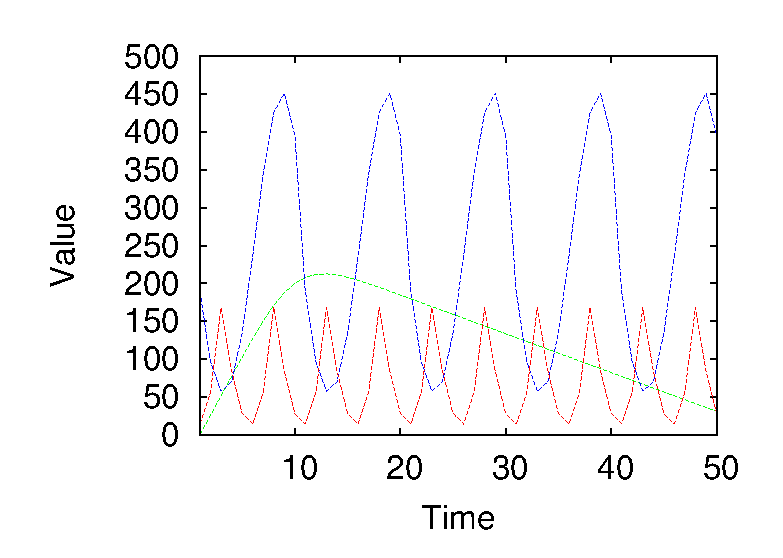
\includegraphics[width=2.0in]{figs/example_compoments.eps}}
\caption{Motivating Example}
\label{fig:example}
\end{figure*} 

% As approximate answers can be computed order-of-magnitude faster than their counterpart exact queries. Therefore, our system support computing approximate queries within error guarantees over future and historic data.

To this end, we introduce a  TimeTravel, an efficient DBMS system for seamless integration  of past and future time series values, supporting two types of queries:
(a)~approximate queries on past and future within user-specified error bounds (i.e., absolute error and confidence), and (b)~exact historic queries.
We can support point, range, aggregate and join queries.
Unlike, previous approaches, we utilize trend and seasonality components to build models over the underlying time series to support . Ignoring seasonality components results in low compression ratio as we will discuss later.  Here, past and future data is treated similarly, allowing seamless integrated querying. The main difference of future data compared to past is that the (estimated) error is typically higher.
To organize these models and efficiently support queries with various error guarantees, we introduce a novel index structure, denoted as {\em \LN}.  The upper levels in the index are more ``coarse-grained'', representing 
the underlying time series with a higher error and a lower confidence and fewer model segments compared to the lower levels which are more accurate. Please note that confidence while building models to reduce the effect of  {\it outliers} on the quality of models.

For approximate historical queries (e.g., last week in our motivating example), we use the highest-level models to calculate an approximate answer. If the  answer violates the user requirements on error and confidence, we consult relevant models at lower levels.  We continue traversing the hierarchical model index until either the error guarantee given by user is met or the underlying time series is accessed.
In addition, TimeTravel efficiently answers exact queries by utilizing the index  to find the relevant portions in the time series. For example, considering MIN aggregation queries, we only access the portion of the time series where the minimum value might exist. 
For future queries (e.g., next week in our motivating example), we use the model index to retrieve forecast states which is supplemented to  statistical forecast methods.
We meet the user required error guarantees on future data by (a)~controlling the error and confidence of the  retrieved forecast states and (b)~optimizing the forecast method parameters. 

To build the hierarchical model index, the user specifies hints for: (1)~seasonality periods, (2)~error guarantees levels, and (3)~the statistical forecast method (e.g., ARIMA).  
We recursively divide the time series into non-overlapping intervals and build a model on each interval until all error requirements are satisfied. 
Over time, {\it new} values are added to the time series, and we incrementally update the parameters for the forecast method and add  models to the hierarchical model index.

In the rest of this paper, first we formalize the problem statements in Section~\ref{sec:form}.   Section~\ref{sec:overview} provides an overview of the our proposed system. Section~\ref{sec:details} describes building the hierarchical model index, and  compression Section~\ref{sec:query} gives the details of query optimization and processing for approximate and exact queries.  The  related work is presented in Section~\ref{sec:related}. Section~\ref{sec:experiments} gives  our experimental analysis for our proposed system   using  both real-world time series data and synthetic data.

%\section{Running Example}
%\begin{figure*}[th]
%\center
%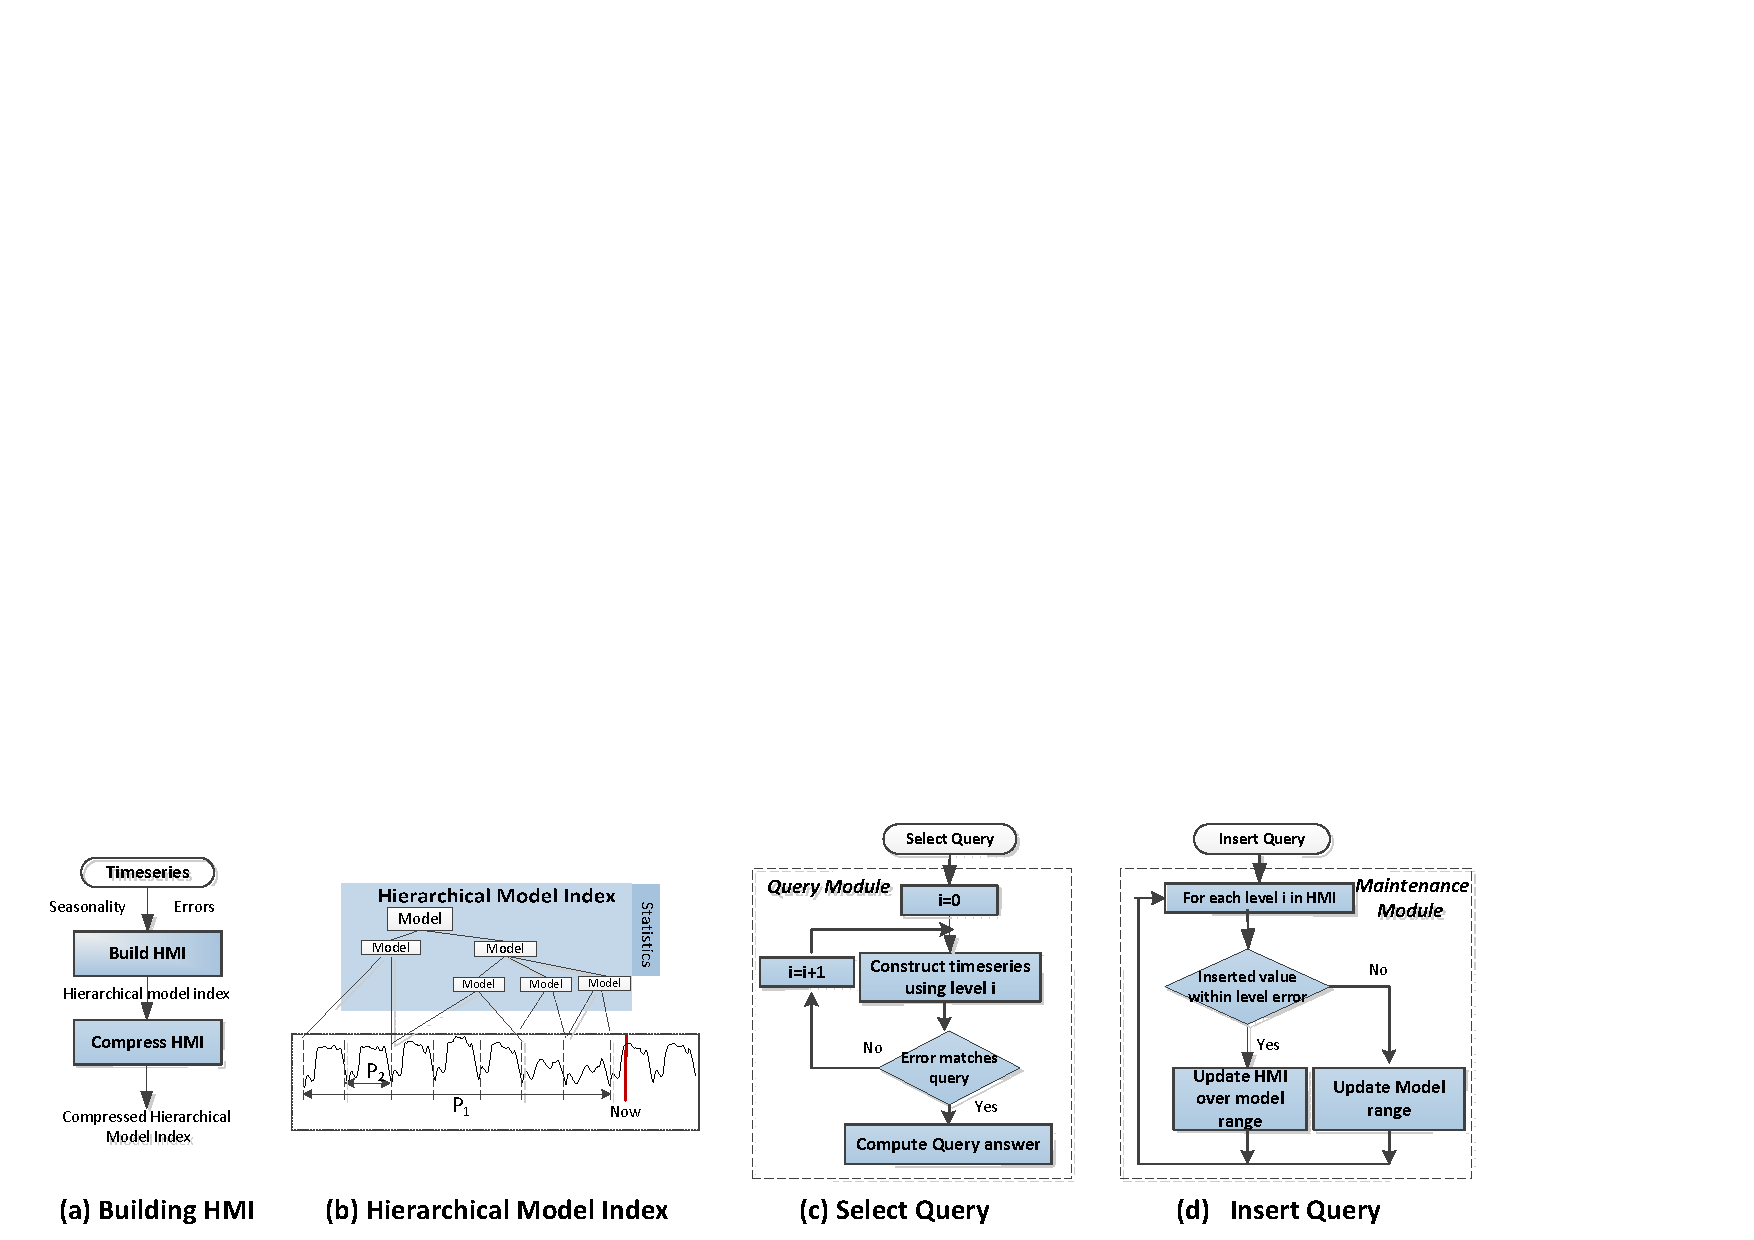
\includegraphics[width=6in]{figs/overview3.pdf}
%\caption{TimeTravel System Overview}
%\label{fig:arch}
%\end{figure*} 
%\begin{figure}[th]
%\center
%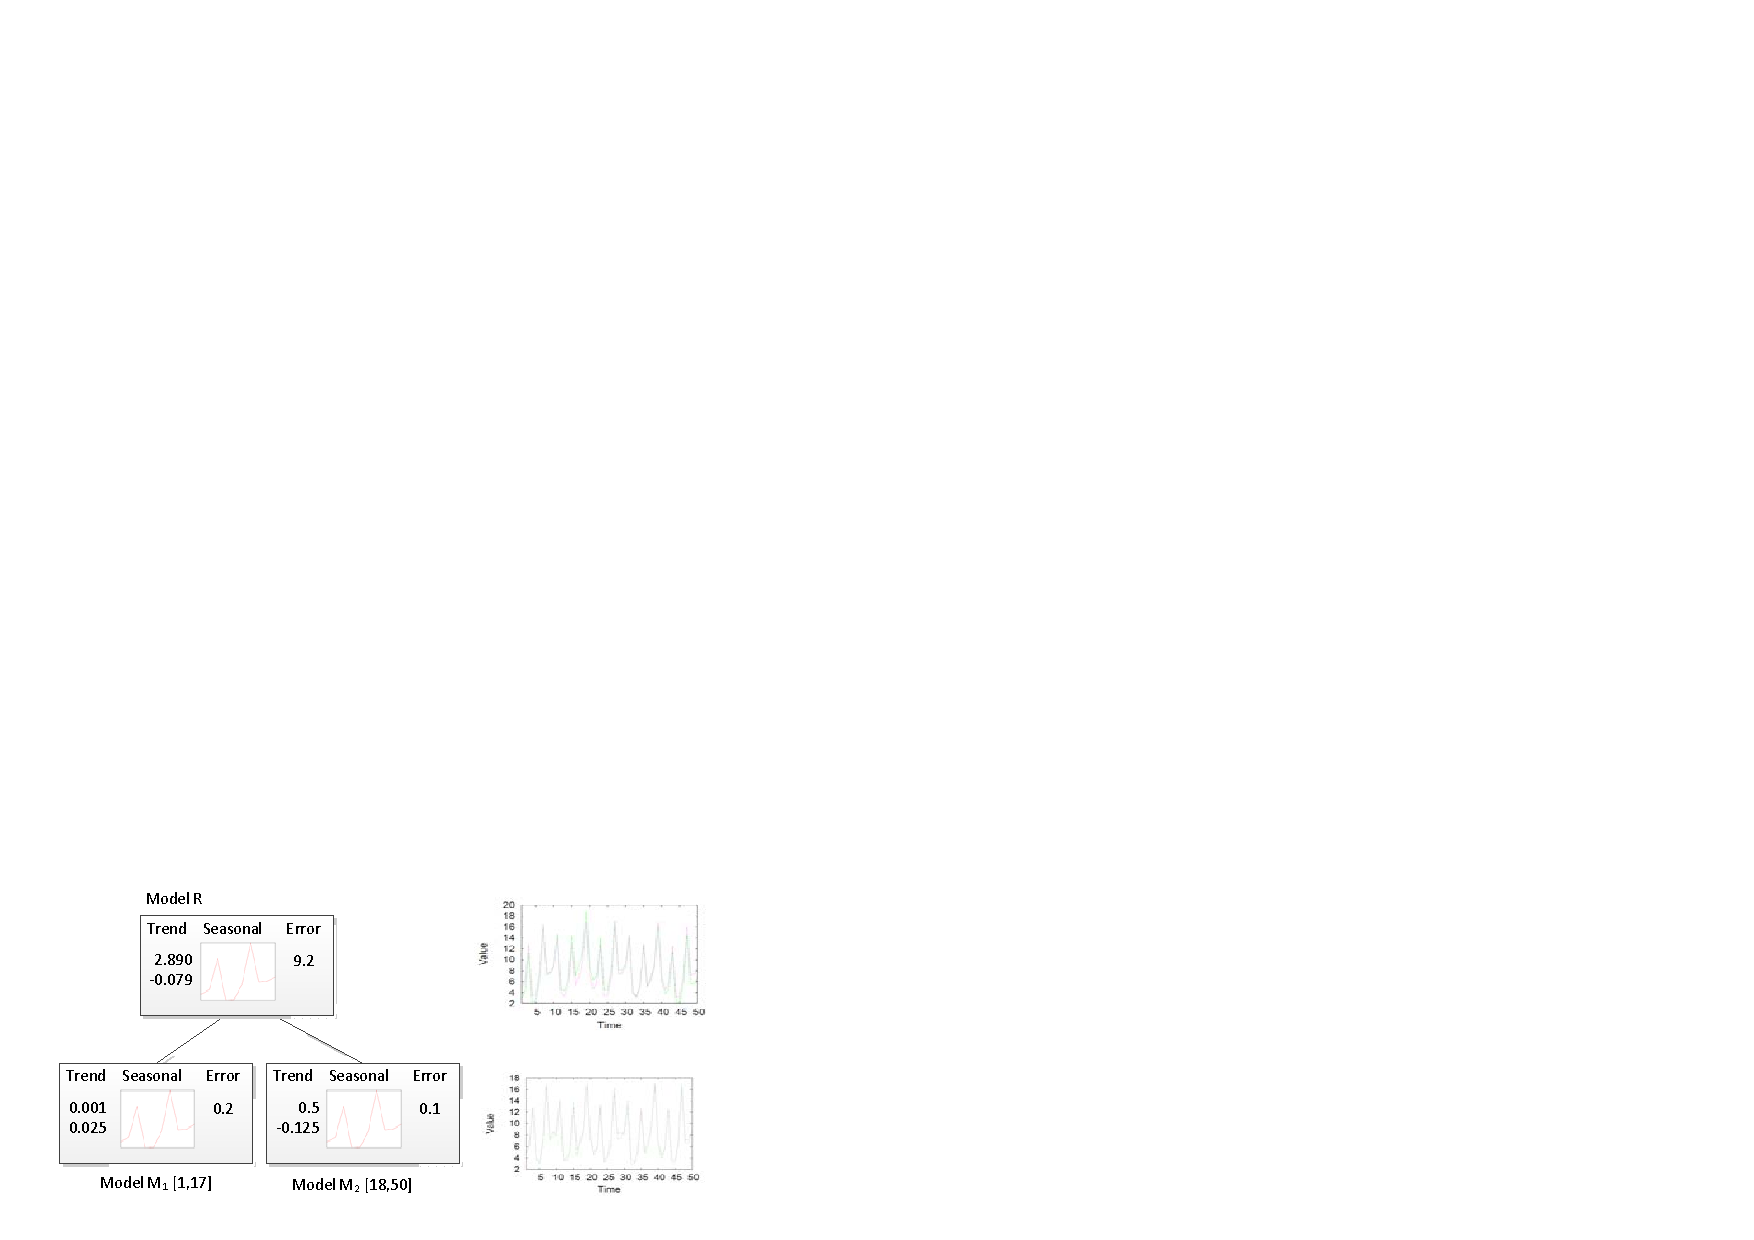
\includegraphics[width=3in]{figs/example_tree.pdf}
%\caption{HMI for the motivating example}
%\label{fig:exampletree}
%\end{figure} 


\section{TimeTravel System Overview}
\label{sec:overview}
Our prototype system, TimeTravel, is implemented {\em inside} the PostgreSQL database engine. For each time series, our proposed system builds a separate model index. The underlying  time series is stored as an array indexed by time.
Figure~\ref{fig:arch} highlights the building HMI module and HMI data structure and Query and maintenance modules of TimeTravel system. These components can be described as follow:

{\em Building HMI} (Figure~\ref{fig:arch}a) First, we  build a HMI  using inputs: (1) Time series, (2)  seasonality periods and (3) errors, and output a compatible \LN.  
The parameters of each model in the HMI are chosen to minimize a heuristic $\cal H$, which is computed as  the product of model's size and its error. This module is invoked offline and presented in Section~\ref{sec:building}.
Then, we reduce the required storage space for \LNs by finding similar models  based on trend and seasonality components. These similar models are combined. The combined model is only stored once which reduces the overall storage. A side effect of  compression is that the increase of the model deviations from the time series (i.e., model error). Compressing the HMI size reduces the run time query as less data are needed to be read from the disk.
The similarity on models instead of the original time series can be computed more efficiently. 

{\em \HMI} (Figure~\ref{fig:arch}b)
  A model  at level $l$ has zero or more children segments at level $l-1$.  Each child model improves its parent's representation of the underlying time series by creating one (or more)  models over a sub range of the timeseries. For example in Figure~\ref{fig:exampletree} the timeseries is divide into two models over [1,17] and [18,50] respectively. To build a child model, we may either use  (a)~sub range of the time series, or (b)~sub range of the error of the parent model. We denote the latter models as $\Delta$Models. 
Figure~\ref{fig:exampletree} illustrates the hierarchical model index for the time series shown in Figure~\ref{fig:example}. Note that the error for models $M_1$ and $M_2$ is greater than zero, because we use only on seasonality component. Also, the error of the root model is greater than both of children models.
A time series can have an arbitrary number of seasonality periods (e.g., the shown time series exhibits two seasonality periods $P_1$ and $P_2$).  The timeseries shown in Figure~\ref{fig:example} has seasonality periods of 10 and 4. The \LNs is presented in the top center of Figure~\ref{fig:arch}.
The HMI has one root node for the entire time series, As we traverse down the HMI the error decreases. 
 For query optimization, we store statistics about the index in the system catalog. Specifically, we store the number of model segments, their average size, and the maximum error and minimum confidence for each level. These statistics are needed to estimate the expected cost for the query.

{\em Query Processing Module.}(Figure~\ref{fig:arch}c) We extend the query processor and optimizer of PostgreSQL to support approximate queries over future and past data and exact queries over the past data. 
To answer historical queries, it traverses down the model index. The Forecasting module is used to retrieve the predicted the time series.
The query processor supports point, range, aggregate, and join queries, as discussed in Section~\ref{sec:online}. 
 The forecasting module is responsible for: (1)~predicting the values of time series for a given future interval, (2)~estimating the error and the confidence of the 
forecasted values, and (3)~reestimating forecast method parameters. It uses the query processing module to retrieve the forecast method states. The error of the forecasted data~\cite{tBOX76a} depends on (1)~the forecast model and the length of forecast data and, (2)~the confidence interval of the retrieved states. Further details are presented in \cite{FRL12}.


{\em Maintenance Module.} (Figure~\ref{fig:arch}d)
The Maintenance module maintains \LNs  when new values are added to the time series.
For each level in the index,  we update the last segment (i.e., the rightmost segment in the figure) with the added values. 
If the error and the confidence of the updated segment violates the model error guarantee, we construct a new segment over the interval of the last model and added values, using the building module, and substitute it for the old one. 




\section{Problem Formulation}
\label{sec:form}
In this section, we give  definitions for our proposed problem. Throughout the paper, we assume a mathematical model to  represent the underlying timeseries. More specifically, to compactly represent a timeseries $TS$ using model  $M_{TS}$, we either: (1)~additively decompose $TS$ into $trend$, $seasonal$ and $error$ using STL algorithm~\cite{STL}. Then, we compute a separate model for each component, or (2)~use explicit values, average  value, or regression line. %
%Move to next We assosicate with each model  minimum and maximum values. 

First, we can formally define a timeseries as follow:
\begin{mydef} TimeSeries: A time series $TS$ is an ordered temporal sequence. $TS$= ($ts_1$, $ts_2$, $\dots$, $ts_n$), where $n$ is time series length, and $\forall_i$ $ts_i$ $\in$ $\mathbb{R}$. Timeseries have a set of periods $\cal P$= \{1, $P_1$, ... $P_m$\} where $m > 0$, and $\forall_i$ $P_i$ is a sequence on the form $k_l$* $P_l$, s.t., $k_l$ $\in$ $\mathbb{N}$ and $l<i$.
\end{mydef}

Timeseries may have one or more seasonal periods. For example, a time series may have  yearly, weekly and daily periods. Weekly periods may divided into five work-days and two weekend-days. Alternatively, we can  divide yearly period directly into work days and week-end days.
 
The mathematical model can be defined as follow:
\begin{mydef} TimeSeries Model: Model $M_{TS}$ for timeseries $TS$ with  $t$, $s$, and $e$ as trend, seasonal and error additive components for timeseries $TS$. i.e.,   
\[
  M_{TS}(t) = \left\{ 
  \begin{array}{l l}
    TS (t) &  \text{;Explicit values}
    \\
    %Mean(TS(t)) & 	\text{;Mean}\\
    %(Min(TS(t)),Max(TS(t))) & \text{;Range} \\
    a*t+b             & \text{;Regression line} \\
    M_{t}(t)+M_{s}(t)+M_{e}(t) &  \text{;Decomposed}\\
  \end{array} \right.
\]
\end{mydef}

The model $M$ does not perfectly match the underlying data, the deviation between the values computed using the model  and actual values is referred to as model errors. The confidence of a model $M$ is the probability that model errors is below certain error level. For example, for 100\% confidence, the error level must match the maximum model errors. We can formally define a  model matching for  error guarantee, as follow:
\begin{mydef} The model $M$ matches error guarantee ($\epsilon$, $\delta$) iff: 
Pr \{ $|(M_{TS}(t) - TS(t)|$ $\leq$ $\epsilon$ \} $\geq$ $\delta$ where $TS(t)$, $M_{TS}(t)$ is the actual and model time series value at $t$, respectively.
\end{mydef}

The goal of our proposed solution is to find models for a timeseries which meet all error guarantees while reducing the size. It can be formally presented as follow:
\begin{mydef} Problem statement: Given: a timeseries $TS$, and error guarantees: ($\epsilon_1$,$\delta_1$),($\epsilon_2$,$\delta_2$)$\dots$, ($\epsilon_m$,$\delta_m$). Find models $M_1$, $M_2$, $\dots$, $M_k$ on the entire or interval of time series $TS$. 
$\forall$ timestamp $t$ in timeseries,  $\exists$ $j$ and $l$ s.t. $M_j$ matches error guarantee ($\epsilon_l$,$\delta_l$) while minimizing the size of all models, i.e.,  $Min(\sum^k_{i=1}{size(M_i)})$.
\end{mydef}


\section{The Hierarchical Model Index}
\label{sec:building}
In this section, we present building and compressing the  Hierarchical Model Index and storing it into PostgreSQL. Finally, we describe incrementally updating the index with the inserting of new values to the time series.% in s  
    %a. Building the Index
    %b. Compression
    %c. Storage? (TimeSeries, ModelIndex) 4. Online  Processing
   % a. Historical Query Processing (Exact, Approximate)
    %b. Forecast Query Processing? (probably quite short)
    %c. Insert Processing (Maintenance)
 
% We introduce a  heuristic, $H$,  to  quantify the  {\em goodness} of a model  in fitting a time series over interval $I$. We define the heuristic  $H$  as $(\sum_{\forall e} {|I_e|})/s$, where $|I_e|$ is the length of interval $I_e$ $\in$ $I$ which complies with the error  guarantees $e$, and $s$ is the model size.
 
%  To build the \LN, we  compute the trend $t$, seasonal $s$, and remainder $r$ components for time series $x$. Then, we process each component  as described  in Sections~\ref{sec:nonseasonal}-\ref{sec:error}. We greedy choose the  presentation of model that maximizes the  heuristic $H$. If the LN does not comply with all error guarantee levels,  we  recursively build  models over sub intervals.
 \subsection{Building the Hierarchical Model Index}
 Add discussion for top down vs bottom up approaches
 
We now describe constructing a \LNs over the time series. The pseudo code is given in Algorithm~\ref{alg:him}. The algorithm takes two inputs: (1)~timeseries $TS$ with seasonal periods hierarchy (we use user hints for seasonality period) and (2)~a set of error guarantees, $error_g$, represented as pair of error and confidence. 
The algorithm finds a hierirehcal model index for the given timeseries such that for each error guarantee, there exists a model (or more) in the index which meets this requirements for the entire timeseries.

Initially, we build one model  over the entire time series. This model represents the root of the index structure. All other models of timeseries (with tighter error gurantess) are  either direct or non-direct children of the root node.
To find the best model representation over entire (or segment of ) time series, we use a utility function defined as the size of the model multiplied by the $\delta$-error  (i.e., the probability that the absolute error of the model is bounded by $\delta$). The utility of the time series is defined to be infinity. The best model for a time series is defined as the model with the smallest utility. 
The algorithm first starts with getting the least error guarantee $(\epsilon, \delta)$. (Line~\ref{alg1:1} in Algorithm~\ref{alg:him})
 Then, we iterate over all periods in the seasonal hierarchy to find best model representation. (Lines~\ref{alg1:s1}-\ref{alg1:e1} in Algorithm~\ref{alg:him})
We decompose the timeseries $TS$ into trend $t$, seasonal $s$, and error $e$ using STL algorithm~\cite{STL}. Then, using FindPossibleTrend and FindPossibleSeasonality (the pseudo code is shown in Algorithm~\ref{alg:t} and Algorithm~\ref{alg:s}), we find possible representations for the trend and seasonality components $t$ , $s$ respectively. 
For each possible representations for trend from  set $\hat{T}$ and seasonality from set $\hat{S}$ (Line~\ref{alg1:ehat} in Algorithm~\ref{alg:him}), First, we compute the error $\hat{e}$ by subtracting the original timeseries from the trend and seasonality representations. (Line~\ref{alg1:ehat} in Algorithm~\ref{alg:him}) Then, we use DivideError algorithm to divide the model error, i.e., $\hat{e}$, into non-overlapping intervals using the error $\epsilon$. The intervals are divided into three categories: (1)~the error of the interval is less than $\epsilon$, (2)~the difference between the minimum and maximum error is bounded by the error $\epsilon$, and (3)~the error of the interval exceeds the threshold error $\epsilon$. (Line~\ref{alg1:divide} in Algorithm~\ref{alg:him}) 
The size of model is computed as the sum of the size of trend and seasonality representations $|\hat{t}|$ and $|\hat{s}|$, and size needed to store the intervals and the minimum and maximum error bound for the model.
(Line~\ref{alg1:size} in Algorithm~\ref{alg:him}) Then, we compute the utility of the model. We use the utility to compare the model with the previous models, keeping the model with largest utility. (Lines~\ref{alg1:u1}-~\ref{alg1:u2} in Algorithm~\ref{alg:him}) 

After finding the model with the best utility, we iterate over all intervals  which is computed earlier using DivideError algorithm in Line~\ref{alg1:divide} in Algorithm~\ref{alg:him} (Line~\ref{alg1:is} in Algorithm~\ref{alg:him}). For each interval, first we  remove from the error guarantees set, i.e., $error_g$, all the error guarantees that are matched. Then, if the interval does not meet all the error guranete, we recursively build two models over the  timeseries and errors in  interval $I$ denoted as $model_I$ and $\Delta model_I$ respectively. (Lines~\ref{alg1:ms}-~\ref{alg1:ds} in Algorithm~\ref{alg:him})
We add the model of interval $I$ with best utility as a child to the model. (Lines~\ref{alg1:u}-~\ref{alg1:add} in Algorithm~\ref{alg:him})
Finally, we return the computed model. 
\begin{algorithm}[tp]
\caption{Creating a Hierarchical Model Index }
\begin{algorithmic}[1]
\Statex Input TS timesreies, $Error_g$
\Procedure{BuildModel}{$TS, ~Error_g $}
\State $(\epsilon, \delta) \gets Last(Error_g)$ \label{alg1:1}
\State $model \gets NULL$ \Comment{best model yet found}
\For {{\bf each}  $period \in TS.period }$ \label{alg1:s1}
\State $(t,s,e) \gets Decompose(TS, period)$
\State $\hat{T} \gets FindPossibleTrend(t, period) $
\State $\hat{S} \gets FindPossibleSeasonality(s,period) $
\For { {\bf each}$(\hat{t},\hat{s}) \in \hat{T}  \times \hat{S} $} \label{alg1:s2}
\State $\hat{e} \gets TS - (\hat{t}+\hat{s})$\label{alg1:ehat}
\State $ Error_{\delta} \gets  (\delta*100)^{th} of abs(\hat{e}) $ 
\State ${\cal I} \gets DivideError(\hat{e})$ \label{alg1:divide}
\State $size \gets |{\cal I}|+|\hat{t}|  +|\hat{s}|+2$\label{alg1:size}
\State $utility \gets  size * Error_{\delta}$ 
\If {$model.utility < utility$ } \label{alg1:u1}
\State $model \gets (\hat{t},\hat{s},\hat{e}, {\cal I}) $
\EndIf \label{alg1:u2}
\EndFor
\EndFor \label{alg1:e1}
\For {{\bf each} $I \in {\cal I}$} \label{alg1:is}
\State ${\cal E}_g \gets Error_g - Matched(model_{best}, I)$
\If {${\cal E}_g != \phi$}
\State $model_I \gets BuildModel(TS[I], {\cal E}_g)$ \label{alg1:ms}
\State $\Delta model_I \gets BuildModel(\hat{e}[I],{\cal E}_g)$  \label{alg1:ds}
%\State $\Delta model_I \gets ISax(\hat{e}[I],{\cal E}_g)$  \label{alg1:ds}

\State $m \gets Best_{utility}(\Delta model, model_I)$ \label{alg1:u}
\State $model.addChild(m)$ \label{alg1:add}
\EndIf
\EndFor 
\State {\bf return} model
\EndProcedure
\end{algorithmic}
\label{alg:him}
\end{algorithm}


%using  , where $|I_e|$ is the length of interval $I_e$ $\in$ $I$ which complies with the error  guarantees $e$, and $s$ is the model size.
 %in Sections~\ref{sec:nonseasonal}-\ref{sec:error}.
 

\begin{algorithm}[tp]
\caption{Find Possible Representations for Trend}
\label{alg:t}
\begin{algorithmic}[1]
\Procedure{FindPossibleTrend}{$T$, $period$}
\State $\hat{T} \gets  \{\}$
\If {$period > 0 $}  \label{algt:ms}
\State // Use Means
\State $\hat{T} \gets \hat{T} \bigcup \{ \frac{\Sigma_{i=1}^{period} {T_i}}{period}, \frac{\Sigma_{i=period+1}^{2*period} {T_i}}{period}, \dots $\}
\State $\hat{T} \gets \hat{T} \bigcup  \{ Mean(T[1:period]), Mean(T[period+1:2*period]),  \dots \} $
\EndIf  \label{algt:me}
\State // Use regression
\State $\hat{T} \gets \hat{T} \bigcup ChebyshevReg(TS)$ \label{algt:cheb}
\State {\bf return} $\hat{T}$\label{algt:r}
\EndProcedure
\end{algorithmic}
\end{algorithm}

{\bf Processing Trend Component}
\label{sec:nonseasonal}
We examine two  trend representations based on means and linear regressions. The pseudo code is presented in Algorithm~\ref{alg:t}. The algorithm takes two inputs: (1) the trend component and (2) the length of the seasonal period. Initially, if the seasonality period is greater than zero,  we present the trend as a vector of  values over each seasonal period. (Lines~\ref{algt:ms}-\ref{algt:me} in Algorithm~\ref{alg:t}) 
We use  the linear Chebyshev regression method~\cite{cheb} to approximate the trend component $T$. (Lines~\ref{algt:cheb} in Algorithm~\ref{alg:t}) The Chebyshev regression method is efficiently computable and 
minimizes the largest deviation (i.e. error) from the original curve (i.e., time series) among the polynomials of the same order. Finally, the algorithm returns possible representations for the trend components. (Line~\ref{algt:r} in Algorithm~\ref{alg:t})
%\begin{figure}
%\center
%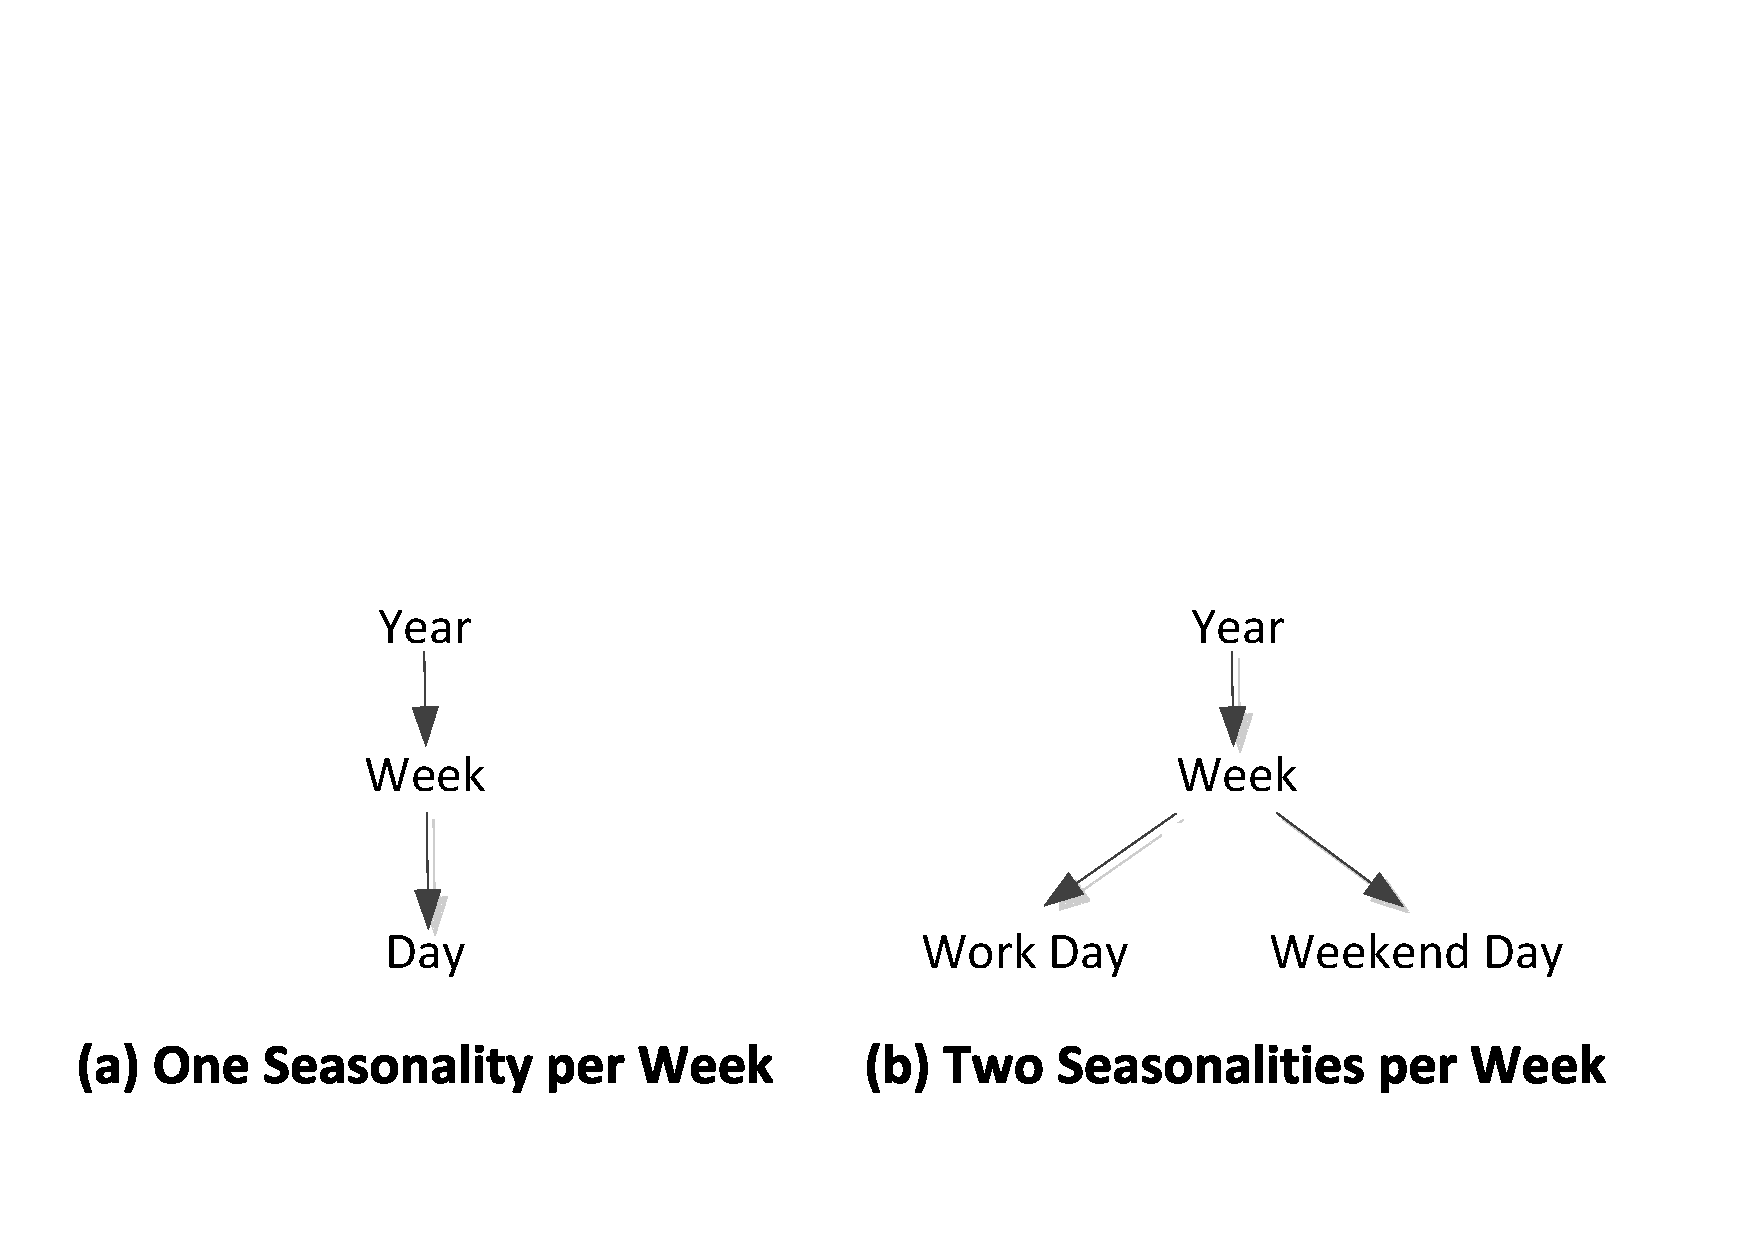
\includegraphics[width=3.0in]{figs/hints.pdf}
%\caption{Possible Hints for Seasonal Hierarchy}
%\label{fig:hints}
%\end{figure}

{\bf  Processing Seasonality Component}
\label{sec:seasonal}
%Trends, seasonality error
Storing the value of each data point in the seasonality component may be expensive (e.g., yearly seasonality).  We may approximate the seasonality component using the user hints by 
recursively calculating the trend and seasonality using smaller seasonality periods. 
The pesduo code for finding possible representations in given in Algorithm~\ref{alg:s}. The algorithms takes two inputs: (1) the seasonality component, and (2) the period seasonality. Please note for this algorithm we need the seasonality  period hierarchy.
Initially, a possible representation is to directly store  data points  of the seasonality component, $S$. (Line~\ref{algs:s0} in Algorithm~\ref{alg:s})
We explore this hierarchical seasonal information to find different representations for the seasonal component. Therefore, we iterate over all the seasonality periods that are smaller than the seasonality period of $S$.
(Line~\ref{algs:s1} in Algorithm~\ref{alg:s})
If the seasonality period consists of  more  than one seasonality period,  for example a weekly seasonality in  figure~\ref{fig:hints}b consists of workday and weekend day, we divide the seasonality into partitions accordingly. (Lines~\ref{algs:s1}-\ref{algs:s2} in Algorithm~\ref{alg:s}) For each seasonality period $S$, we decompose it into three components $(S.t,S.s,S.e)$. Then,  we use FindPossibleTrend over the computed trend $S.t$ and recursively use FindPossibleSeasonality for the computed seasonality component $S.S$. For each possible representation for trend and components, it is added to the possible seasonal representations  (Lines~\ref{algs:s3}-\ref{algs:s4} in Algorithm~\ref{alg:s}) Finally, we return the set of possible seasonality representations. 
%We use the hints for seasonality given by the user to efficiently store the seasonality component. 
%To find the best approximation for seasonality, we utilize the heuristic described above. 
 
%{\bf Processing Error Component}
%\label{sec:error}

%As regression and seasonality model does not perfectly fit the input time series, errors exists. 
%Error is computed as $x$-($\hat{t}$+$\hat{s}$), where $x$ is time series  over interval $I$, and $\hat{t}$ and $\hat{s}$ are the stored model  values for the trend and seasonality components, respectively.
%We split the error values into at most $k$ intervals on the time dimensions, where $k$ a system parameter representing the maximum fan-out in the model index. For each interval, we can either (1)~apply a data clipping techniques (e.g., \cite{isax2}), (2)~ store upper and lower error bounds, or (3)~fitting a model (i.e., $\Delta$Model) to the error.

\begin{algorithm}[tp]
\caption{Find Possible Representations for Seasonality}
\label{alg:s}
\begin{algorithmic}[1]
\Procedure{FindPossibleSeasonality}{$S$, $period$}
\State $\hat{S} \gets  \{S\}$ \label{algs:s0}
\For {{\bf each} $ p \in TS.periods, s.t., p< period$}
\If {$p$ contains more than one period} \label{algs:s1}
\State ${\cal S}\gets                DivideTimeseries(S,p)$
\Else 
\State ${\cal S} \gets S$
\EndIf\label{algs:s2}
\For {{\bf each} $ S \in {\cal S} $}     \label{algs:s3}
\State $(S.t,S.s,S.e) \gets Decompose (TS, p.period)$
\State $\hat{S} \gets \hat{S} \cup FindPossibleTrend(S.t) \times FindPossibleSeasonality(S.s)$
\EndFor \label{algs:s4}
\EndFor
\State {\bf return } $\hat{S}$
\EndProcedure
\end{algorithmic}
\end{algorithm}


\subsection{Index Compression}
We can reduce the the size of hierarchical model index while meeting the error guarantees. This is based on that  the error and confidence for some models are  lower than  the user-specified error guarantees. Several algorithms 

Algorithm~\ref{alg:c} gives the pseudo code for compressing the hierarchical model index, it takes the model index and error guarantees as inputs.
First, we iterate through similar models in the model index. The similarity for two models $M_i$ and $M_j$ are  in relative to trend and seasonality representations. Please note that we normalize the representations for both models to find the similarity. (Lines~\ref{algc:c1}-\ref{algc:c2} in Algorithm~\ref{alg:c}) Then, we use $M_i$ to compute data points over the range of model $M_j$. If the error and confidence for the computed data points is within the error guarantee for model $M_j$, we drop $M_j$ from the $HIM$, and use denormalized $M_i$ instead. (Lines~\ref{algc:c3}-\ref{algc:c4} in Algorithm~\ref{alg:c}) Similarly, we check if model $M_j$ can be used to compute the data points of model $M_i$. (Lines~\ref{algc:c5}-\ref{algc:c6} in Algorithm~\ref{alg:c}) Otherwise, we build new model $M_{ij}$ over data points of models $M_i$ and $M_j$. $M_{ij}$ can be used only if the error guarantees are matched for both $M_j$ and $M_i$. (Lines~\ref{algc:c7}-\ref{algc:c8} in Algorithm~\ref{alg:c})
\begin{algorithm}[tp]
\caption{Compressing The Hierarchical Model Index}
\label{alg:c}
\begin{algorithmic}[1]
\Procedure{CompressingModelIndex}{$HIM$, $error_g$}
%\State ${\cal M }\gets sort(Models \in HIM)$ \label{algc:c0}
\For {{\bf each }$ similar~ models~  M_i, M_j \in {\cal M}$ } \label{algc:c1}
\State $TS^i_j \gets  M_i(TS_j)$ \label{algc:c2}
\If {$\epsilon(TS^i_j)$ is within error guarantee of $M_j$} \label{algc:c3}
\State Replace $M_j$ with $M_i$ in $HIM$ 
\State Delete $M_j$ \label{algc:c4}
\ElsIf{$\epsilon(TS^j_i)$ is within error guarantee of $M_i$} \label{algc:c5}
\State Replace $M_i$ with $M_j$ in $HIM$
\State Delete $M_i$ \label{algc:c6}
\Else 
\State $M_{ij} \gets BuildModel(TS_i \cup TS_j, error_g)$ \label{algc:c7}
\If{$ error of M_{ij} matches M_i and M_j$}
\State Replace $M_j$ and $M_i$ with $M_{ij}$ in $HIM$
\State Delete $M_i$; Delete $M_j$ \label{algc:c8}
\EndIf
\EndIf
\EndFor
\EndProcedure
\end{algorithmic}
\end{algorithm}



\subsection{Storage}
 A system catalog table, $PG_{HIM}$, is added to store the information needed about hierarchical model indexes. We extend the relation  to store the  model index, the first tuple in the first page corresponds to the root of the model index. Each entry in the catalog table contains: (1) The attribute in the base relations, and (2) the relation used to represent the hierarchical model index. In addition, we store in system catalog, $PG_{eg}$,  for each error guarantee, the needed number of page access in its model index.
 
To natively store the described model index in PostgreSQL, we extended the page layout to be able to efficiently store this recursively data structure. We store the model header which consists of: (1) model type (i.e., delta model, normal model), (2) the minimum and maximum error, (3) the range where the model is valid, (4) the number of children models with pointer to model index, (5) the trend representation, and (6) the seasonality representation which may be recursively represented. 

 %To find best models at each level, we use a heuristic to quantify the  {\em goodness} of model $m$ in fitting the time series $x$. 
 
 %the And find the presentation that maximize the  %Several heuristic (e.g., ~\cite{functionDB} and \cite{Shatkay}) can be used to divide the interval $i$ into sub intervals. including approaches. 
  
 %Let $x$ be  and $\hat{x}$ be the time series and approximation. 
 
%Let the maximum branching factor for models be  $K_{max}$ and the levels of  error guarantees  be ($E$,$\Delta$)=($\epsilon_1$, $\delta_1$), ($\epsilon_2$,  $\delta_2$), $\dots$. 
%We find up to $K_{max}$ intervals $I_1$, $I_2$, $\dots$, such that we maximize $\sum{|I_i|^2\frac{\delta_i}{\epsilon_i}}$, where $|I_i|$ is the the length of  interval $I_i$ and $\exists$ ($\epsilon_i$, $\delta_i$) $\in$ $E\cup(\infty,0)$, s.t. $\delta_i$ and $\epsilon_i$ are the lower and upper  bound of confidence and error of model $m$ on interval $I_i$. 
%If the error and confidence matches the minimum error and maximum confidence in $E$, no further processing is needed.
%Otherwise, we remove from $E$ all error guarantees that are stratified by  model $m$, and recursively build a new model whether error model or  over each intervals.

%new level is needed if the error of the last model does not comply the minimum errro guranteee
%We divide the error into two sets of intervals $I_g$ and $I_l$ for intervals with   error greater and lower than the error $\epsilon$, $I_g$ and $I_l$ respectively. 
%Then, for each intervals in $I_g$, if the difference of the  maximum and  minimum errors in this interval is less than $\epsilon$, we add these intervals to $I_l$.
%Otherwise, we divide each  interval in $I_g$ into two intervals using the point with the maximum error, and add them to $I_g$.
%If the number of intervals in $I_l$ and $I_g$ are greater than $K_{max}$, we repeatly combine adjacent intervals. If the error qurantee of the combined  and compute the error and confidence of the combined interval 

%%{\bf Dividing Interval}. As discussed earlier, we divide interval $I$ if $max(e\in I )-min(e\in I ) > \epsilon$, and the confidence is lower than $\delta$. More specifically, to split an interval $I=(f,l)$, where $s$, $e$ are the first and last index respectively,  into $k$-smaller intervals: 
%%We split  interval $I$ into $k$ intervals $I_1=(f,x_1)$, $I_2=(x_1,x_2)$, $\dots$, and $I_k=(x_{k-1},l)$, such that $x_1$$<$$x_2$$<$$\dots$$x_k$.   Then, we build a model for each interval. The goal is to find $i_1$, $i_2$, $\dots$, $i_k$ which minimizes the total sum of absolute error for each interval.
%each possible represntation and choose the rerepeseantion with the higest
%Basically, er approximate the seasonality using $s$
%Please note model $m$ stores  $\hat{s}$ which approximates the seasonality component $s$.
 %exists within the  seasnoality compoment. over  using smaller periods (e.g., week  build a model  For seasonality period $p$ within interval I over time series $x$, we compute the trend $t(x)$, seasonal $s(x)$, and error $\epsilon(x)$ components.  For trend, seasonality, and error components, we either store or model the values of the component using approaches sections~\ref{},~\ref{} ,~\ref{}, respectively. For  seasonality component, if there is a period $p'$ within period $p$, we recursively  model  the seasonality  with period $p'$, otherwise we use non-seasonality  modeling.
 
% For example, the power usage differs for week day and weekends.

 

%To be able to answer approximate answer within the user-defined error and confidence, these modeling errors should be modeled. The main idea  is  to identify the intervals where absolute error  exceed the user model. For these intervals, we create more detailed models.

%With respect to  error level $\epsilon$ and confidence $\delta$ over the interval $I$, we have three possible cases: (1)~$ max_{i\in I}(e_i) < \epsilon$. In the case, the model fits the time series data, and no further processing is needed. (2)~$max_{i\in I}(e_i)-min_{i\in I}(e_i) < \epsilon$. In the case, we store the  minimum  error, no further computations are needed, or(3)~$max_{i\in I}(e_i)-min_{i\in I}(e_i) > \epsilon$.
%In the case, the span of the error  over interval $I$ exceeds the error level.
%We keep removing the data points with the maximum absolute error from this interval until (a)~the confidence is violated, i.e., the ratio of the remaining points is less than the confidence $\delta$. Hence, we divide the interval $I$ into  smaller intervals and build a model over the points for each one, or (b)~the remaining points satisfy either case~(1) or case~(2). 
%We store the minimum error $min_{i\in I}(e_i)$, and a pointer to the model, if any.


%Figure~\ref{fig:a} shows intervals of error for fitting model over  time series from Figure~\ref{fig:data}. As shown, interval $I_1$ and  $I_2$ has er

%\subsection{Compressing The Model Index}
%\label{sec:compression}
%To reduce the storage requirements for the hierarchical model index, we combine  similar models. Two models are similar if the difference metric between their corresponding trends and seasonality values are within a certain threshold.  More specifically, consider models  $M_a$ ,$M_b$ on interval $I_a$, and $I_b$ respectively. First, we align  intervals $I_a$ and $I_b$ to have the same starting point. Then, we compute a model $M$ using the values of time series data from  intervals $I_a$ and $I_b$ with the time dimensions is shifted. If the error and the confidence of the model $m$ over intervals $I_a$ and $I_b$ within the same error and confidence level for models $M_a$ and $M_b$, we (1) discard models $M_a$ and $M_b$ from the model index. (2) store one copy of $M$, and the time shift values for intervals $I_a$ and $I_b$.
% Please note that we still need to store two different error components for  each model.
%More generally, we store the difference in the 
\section{Query Processing}% \& Optimization}
\label{sec:online}
In this section, we describe query processing and optimization for point, range, aggregate, and join queries over past or future data for approximate and exact queries.
The underlying time series is stored as an array indexed by the time attribute.

To completely incorporate the model index into Postgres, we extend the query optimizer to estimate the expected cost of queries using the proposed model index.  Specifically, we add to the system catalog statistical information for average model size, number of model segments, the span of the seasonality component, 
and the maximum error and minimum confidence for each level in the model index. Moreover, we store  the number of data points of the time series that fits in one page.
By using this information, the query optimizer estimates the cost of executing a query using the model index or directly using the stored time series,
and creates the query plan accordingly.
As mentioned in \cite{ArimaDB}, the dominant cost of forecast queries is re-estimating the forecast model parameters. Unfortunately, the burden of this cost cannot be avoided. 
However, we only reestimate the parameters if necessary\cite{FRL12}, and the cost is amortized over the query workload. For simplicity, we do not include it in our cost model.

The general idea of query processing is to construct an approximation for the time series using the models and the error guarantee. Each value is represented as an 
uncertain range $[v+l,v+u]$, where $v$ is the value from the model, and $l$ and $u$ are the lower and upper bound of the error, respectively.
The approximation can be arbitrarily improved by traversing down the index. An important optimization is that we use the model parameters, span of seasonality, and error to find the relevant portion of the time series. %Moreover, we progressively read the seasonality component (e.g., using year  to further increase the accuracy of the approximation. 
%We   An upper bound cost for computing the value of a  data point using the hierical index model is easy to compute by storing the maximum error and minimum confidence for each level in the hiereicy. Let $n_l$ be the number of the  models at level $l$.

{\bf Point Queries.}
As the underlying time series is stored as an array, we need at least one page access to find the value of the time series for any point in the past, with 0\% error and 100\% confidence,  
while for forecast queries, we access the forecast model parameters and states (i.e., historic values). We estimate the cost of finding the values of the historic data either using the time series or using the index structure.
 
%For a query $Q$ with range $r$ over historic data with maximum error $\epsilon$, minimum confidence $\delta$, 
% we find level $l$ such the the error of $l$ is smaller than or equal to $\epsilon$, and the confidence of $l$ is greater than or equals to $\delta$. The expected cost of  model index at level $i$, $c_i$, equals to  $\frac{r}{R}$*$n_i$, where $R$ is the range of the time series, $n_i$ is the number of models at level $i$. Hence, the expected cost of  query is the total sum from level $n$ to level $i$, i.e., $cost(Q)$=$\sum_i^{n}{c_i}$. While the cost of directly use the time series is  $\frac{r}{b}$, where $b$ is the number of data points of the time series that fits in a page.
 {\bf Range Queries.}
 We use the system catalog statistics to estimate the cost of a range query. We accomplish this by computing an upper bound on the number of model segments in the requested range 
at each level in the model index. While the cost of directly using the time series is  $\frac{r}{b}$, where $b$ is the number of data points per page, and $r$ is the query range.
To compute any future data point for forecast queries,  we need to retrieve the relevant forecast states, i.e., to answer a range query $Q$ in the future, we need to compute range queries over the past to get all states. To this end, we can estimate the expected cost for forecast range queries by either  using the model index  or accessing the underlying time series directly. 
Processing a  range query $Q$ can be presented as follows: we traverse down the  model index, discarding  model segments that do not overlap with the specified range $r$ until we reach level $l$ that matches the user requirements of error and confidence.

%For query optimization, we use the same cost model, as aggregate queries. 
{\bf Aggregate Queries}
The query processing and cost estimation for an aggregate query depends on the type of aggregate function used.
For MIN/MAX aggregates, we use the approximated representation of the time series to  identify  possible intervals (i.e., ranges) within the query range where the  minimum (maximum) may exist, 
discarding most of the range of the query.
For SUM/AVG aggregates,  a nice property of linear regression is that the total sum of the errors equals zero. Hence, while traversing the hierarchical model index, we discard an interval $l$ from further processing, if we encounter a model segment $m$ over interval $l$ that fully overlaps with the range of the query.

{\bf Join Queries.}
For simplicity, we limit our discussion to equi-join queries. 
Joining the time series $x$ and $y$ over the time attribute can be performed as follows: we progressively traverse the indexes for time series $x$ and  $y$. If the error of the combined results exceeds the query requirements, we increase the accuracy of join results by traversing down the index  with the maximum error.
 For joining time series on a value attribute, we build an approximate representation for each time series using the model index.  
For each potential intersection (i.e., join output), we eliminate false positives by traversing down the corresponding model index.

\section{Related Work}
\label{sec:related}

MauveDB~\cite{MauveDB} proposed  querying models using a relational framework for sensor data.  FunctionDB~\cite{functionDB} supports regression functions to represent the data. Queries on these function are processed using an algebraic solver.
Pluse~\cite{pluse} is a continuous stream query `processor that can fit one-dimensional functions. It finds the query results by computing the algebraic solution to systems of equations. It back-propagates the query result to validate the error on the input. In comparison, in TimeTravel, we directly associate the model with error and hence can bound the error of the answers. 
 To answer approximate queries Shatkay~\cite{Shatkay} proposed  an algorithm to fit a curve using a set of lines or Bezier curve while bounding the error.
All of these approaches uses only regression functions. Ignoring  seasonality significantly increases the number of needed regression functions. MauevDB and functionDB do not give any error guarantee, nor support forecast queries. In comparison, TimeTravel supports more powerful functions, seasonality, and error guarantees. 

On the other hand,  ISAX~\cite{isax,isax2} and data clipping~\cite{clipping} approximate the time series by mapping each value in the time series to a value in a much smaller domains (e.g., a domain of two values in~\cite{clipping}). 
Unlike our approach, the error of   depends on the cardinality of the mapped domain and the compression ratio.

similarity not 
%\balance
%Pluse proposes  a query inversion to bound the  error of query results which is one 
%\section{Demonstration Scenario}
%\label{sec:demo}
%TimeTravel is based on PostgreSQL and integrates
%the different modules described in this paper. Our demonstration
%shows building  the \LNs for real-world time series, and the effect of varying the error guarantees on the speed up of approximate and exact queries.
%The user specifies the seasonality hierarchy,  error guarantees and the statistical forecast method using a graphical user interface.


% The user can browse the hierarchical index and update model  parameters.  
% We show the scalability of our system, and the speed up for approximate queries and  exact queries using the index.

%{\bf Time series} We will use several real-world
%datasets to demonstrate our system. We mainly use the UK household power consumption time series and 
%Australian  tourist visitors nights.
%. In addition, we provide a real-world time series for the number of cars 
%at a certain intersection and visitor nights for Australian  tourism. 
%will provide , traffic one dataset was obtained from the Tourism Research Australia (http://www.ret.gov.au/tourism/tra/domestic/national/Pages/default.aspx) and consists of observations on the number of visitor nights for the Australian domestic tourism according to different countries and purposes of visit. In addition, we will provide real-world datasets from the energy domain. These datasets pose the challenge of high update intervals and demonstrate the necessity of our lazy maintenance scheme.


%\begin{figure}
%\center
%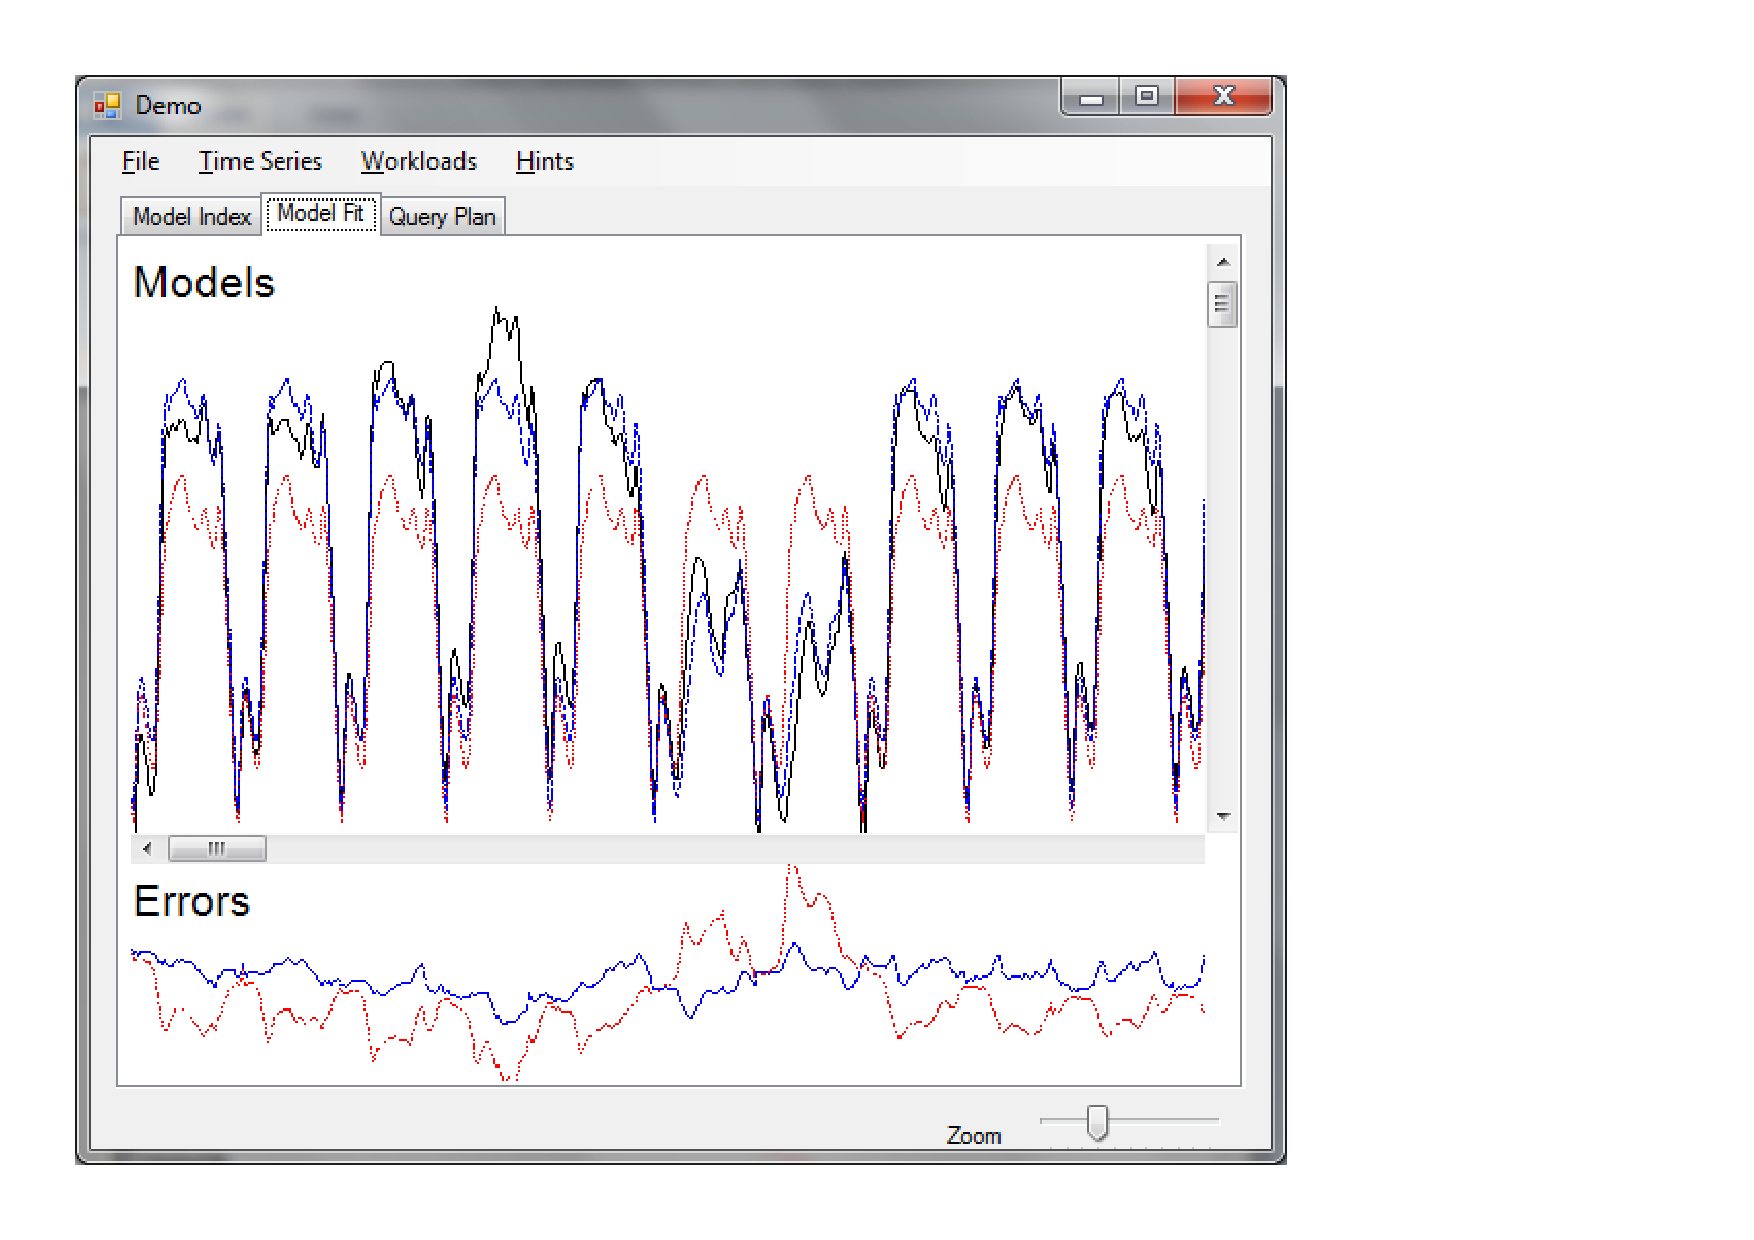
\includegraphics[width=2.8in]{ss1.pdf}
%\caption{Model Fit \& Errors for level 1 \& 2}
%\label{fig:fit}
%using Seasonality Hierarchy from Fig~\ref{fig:hints} 
%\end{figure}
%We canned different configurations to illustrate this effect of changing these values. For each configuration the system computes the expected speed up for the given workload and the storage space needed by the model index.
 
%{\bf Scenarios} The prototype is divided in three different
%aspects: (1) model index view, (2) model fit view, and (3) query plan view. 
% Using the model index view,  we illustrate building a \LNs using the user hints. A demo user can browse the resulting \LN.  She may change the heuristic function used, or directly update model parameters (e.g., intervals, regression line, or seasonality). The user can interact with  the compression module by combining and separating model segments. For the purpose of the demo, the demo user can submit different query workloads. For any change in the \LN, we estimate the response time for these query workload, as well as, the total storage space.
   
% By using the model fit view, the demo user can investigate how the model fits the time series using different levels of the hierarchy by displaying the models versus the time series and/or plotting the error component.
% Figure~\ref{fig:fit} shows a screenshot of model fit and error using models at level $1$ and $2$. The time series used is two weeks from UK household power consumption.  The black line represents the original time series, while the red dashed lines uses model segments at level $2$ which uses the seasonal hint (Figure~\ref{fig:hints}(a)). The blue dotted line shows the models at level 1, which splits the week into workdays and weekend days (Figure~\ref{fig:hints}(b)).
%As time passes, we show how the expected future data generated from forecast method fits the actual data, and how updates affect the model index.
 %we can update From a global point of view, a user can view and manipulate the model pool by using our model index (Figure 2). Different workloads can be submitted to our system and statistics like the maintenance cost, forecast accuracy or query throughput can be viewed. This is also an interactive part where the demo visitor can change workloads (e.g., query and insert frequency) and parameters (e.g., model types, maintenance strategy). In addition, we prepared some demo runs in order to benchmark different model configurations (e.g., all possible models vs. advisor recommendation) in terms of average forecast accuracy and query throughput.

%Last, we will show the query plan for a set of approximate and exact queries given by the user.  For each query, we show the tradeoff between query cost and the error guarantee.
\section{Experiments}
%\begin{figure*}
%\center
%\subfigure{
%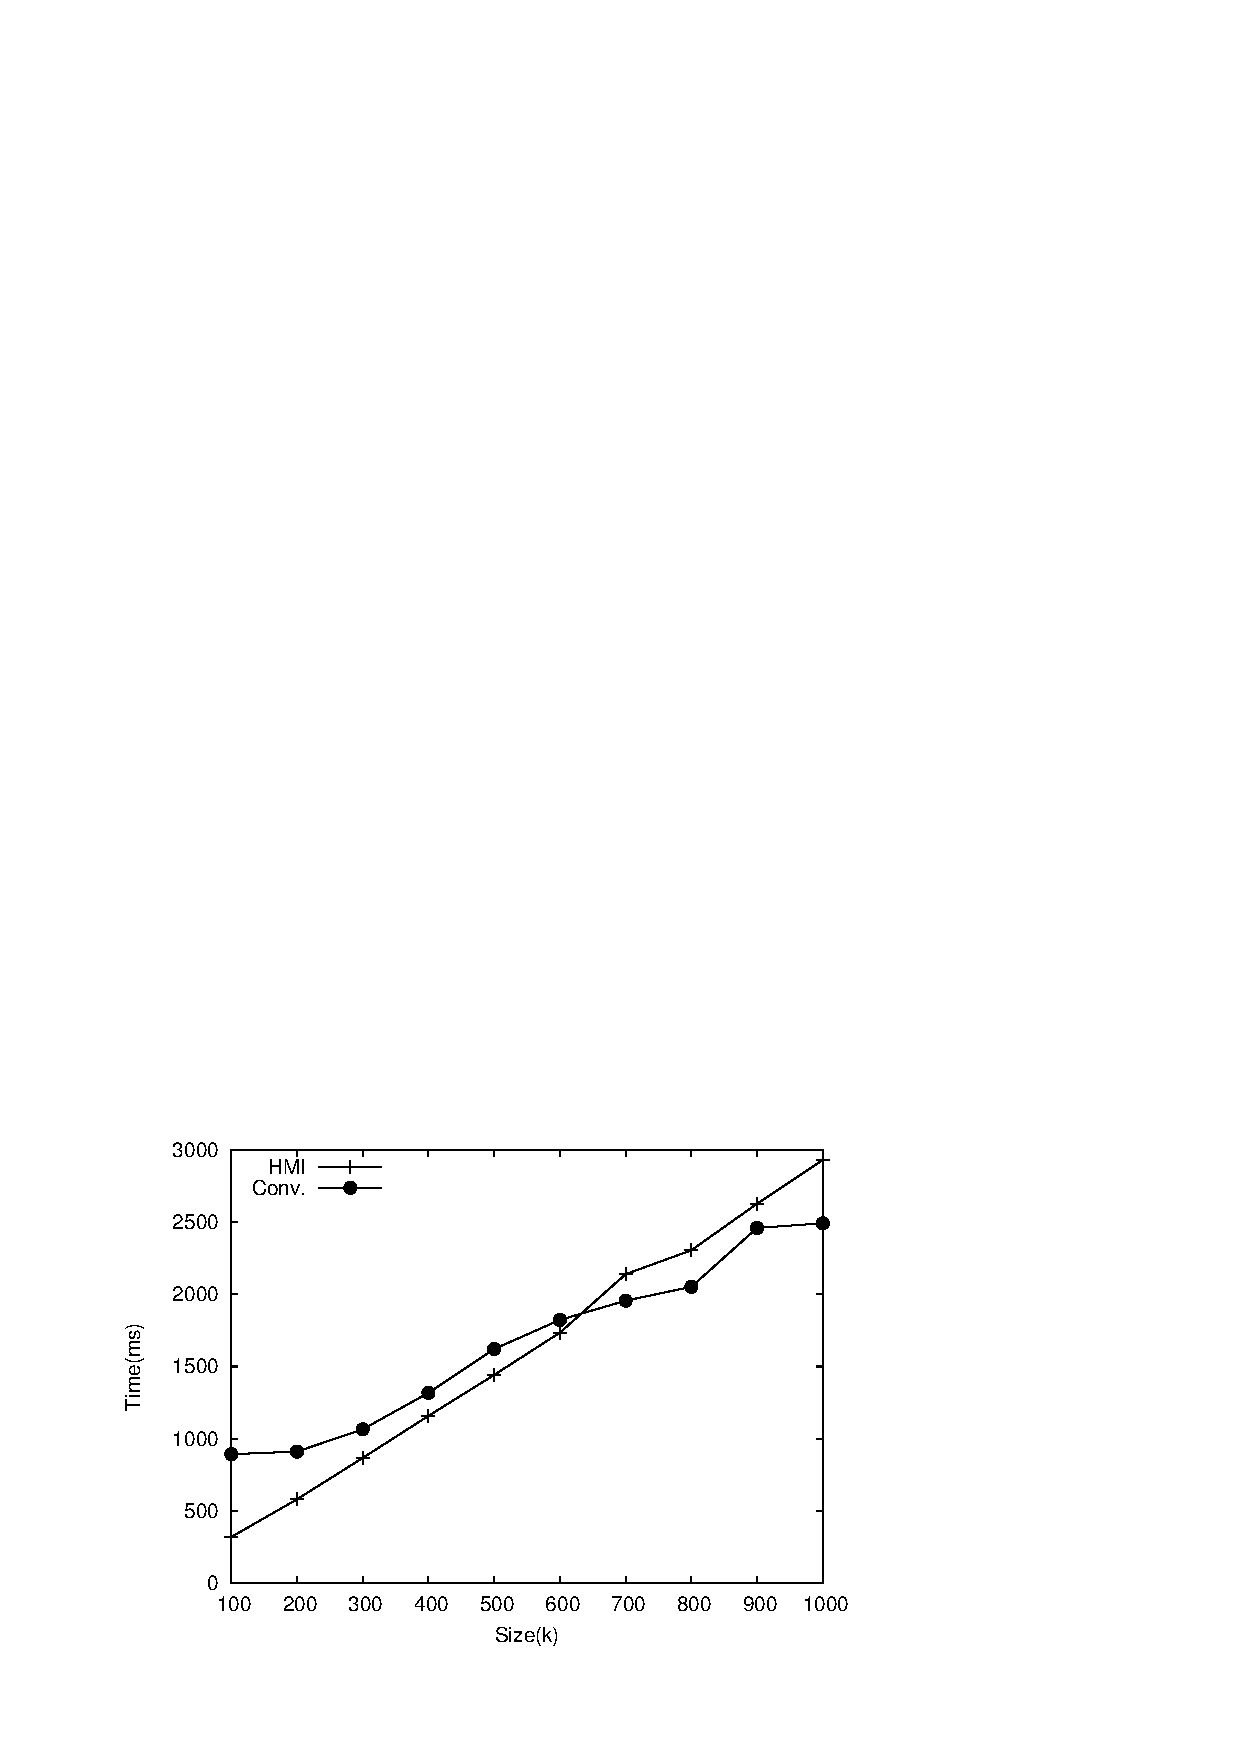
\includegraphics[width=1.5in]{figs/expr/pdf/g_scal_l1i1.pdf}}
%\subfigure{
%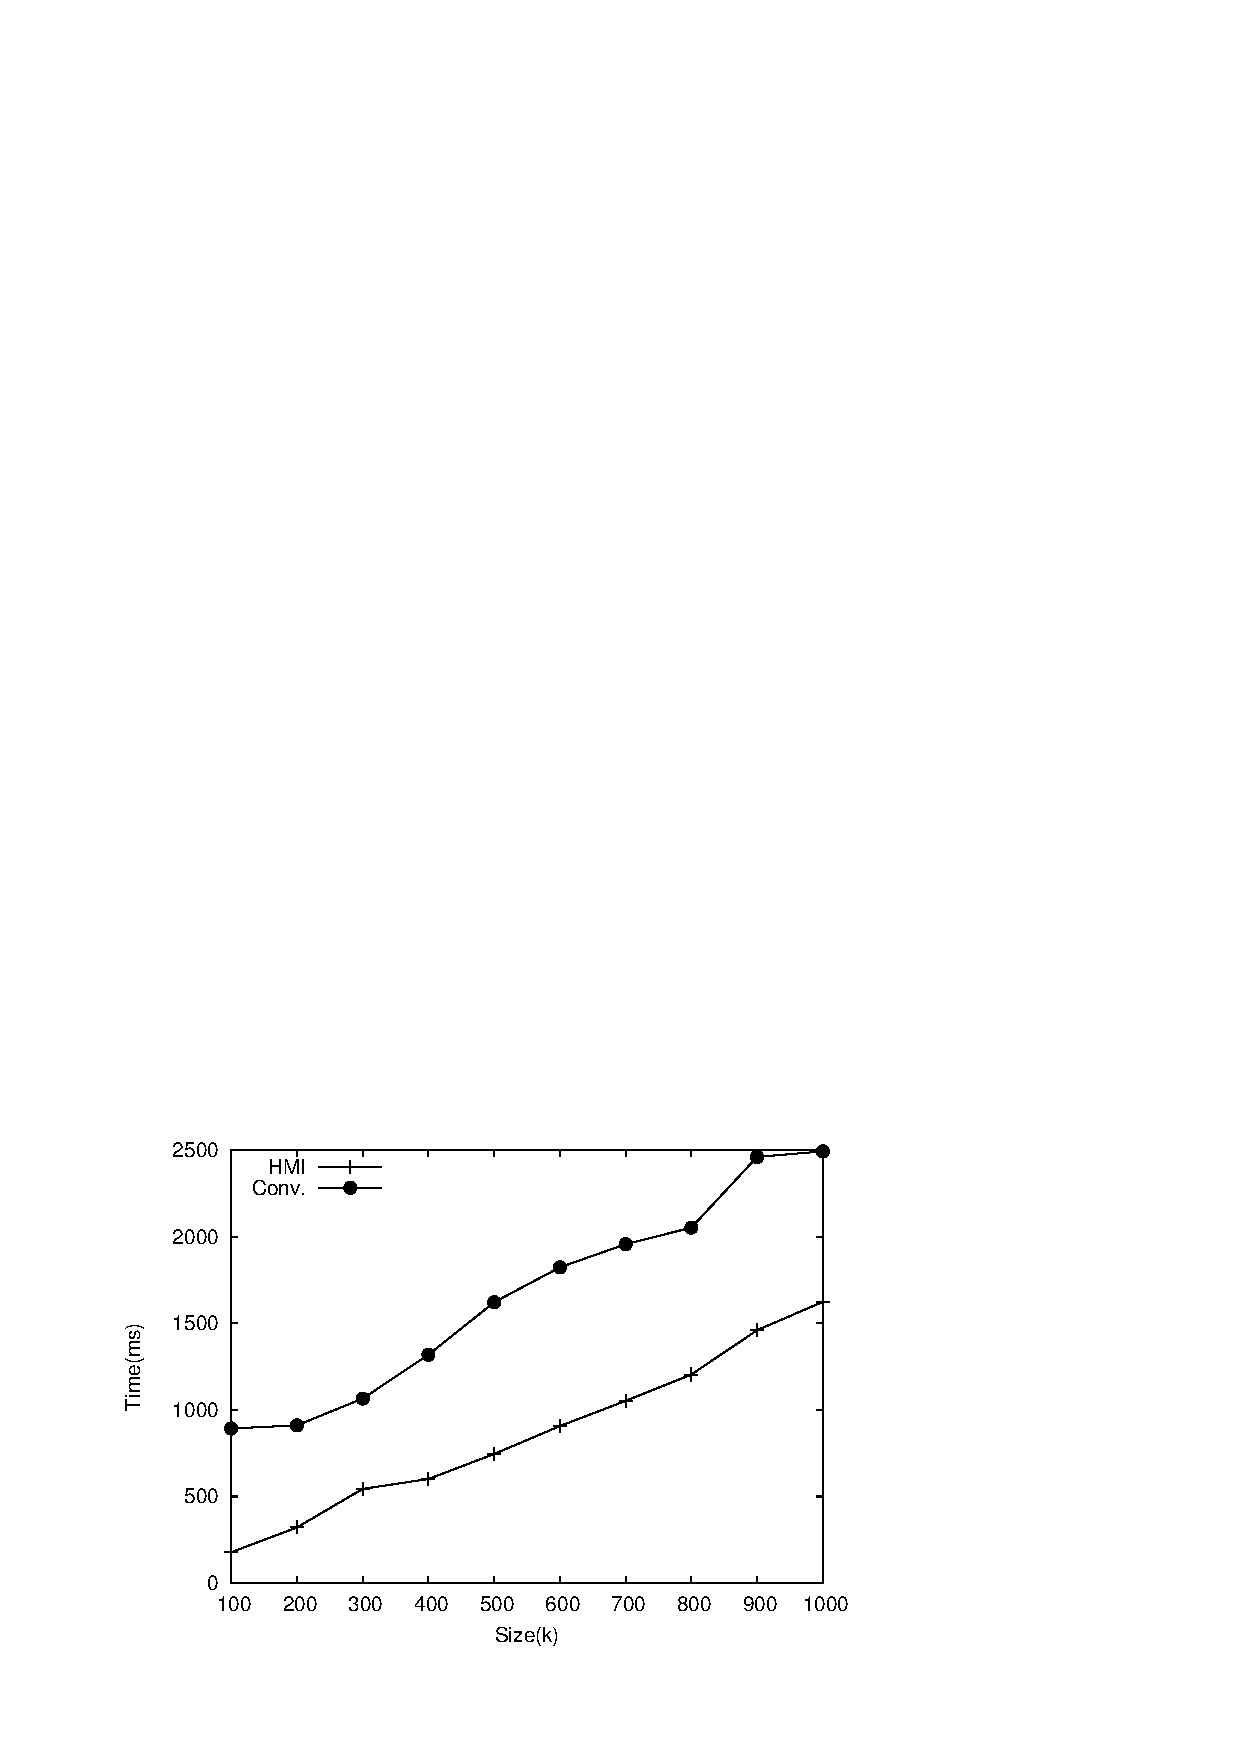
\includegraphics[width=1.5in]{figs/expr/pdf/g_scal_l1i2.pdf}}
%\subfigure{
%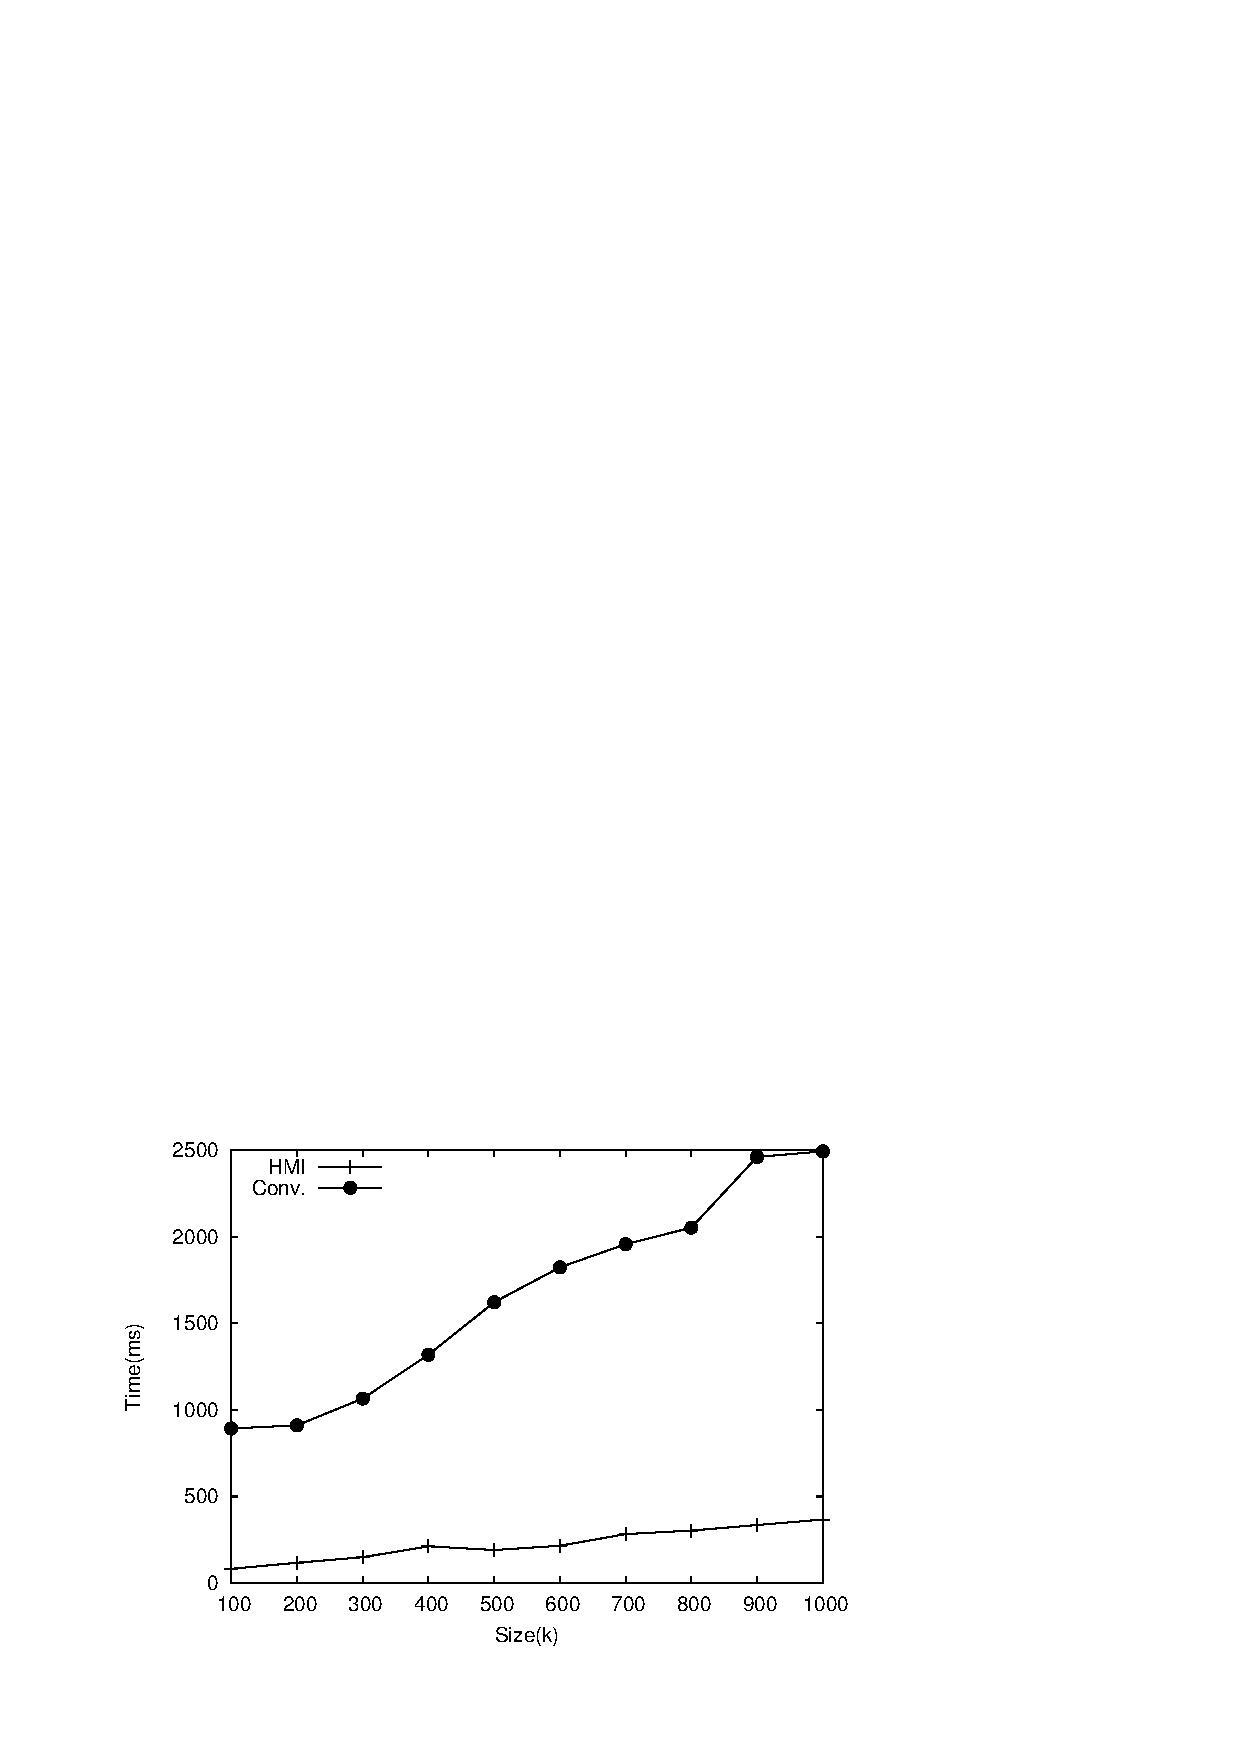
\includegraphics[width=1.5in]{figs/expr/pdf/g_scal_l1i10.pdf}}
%\subfigure{
%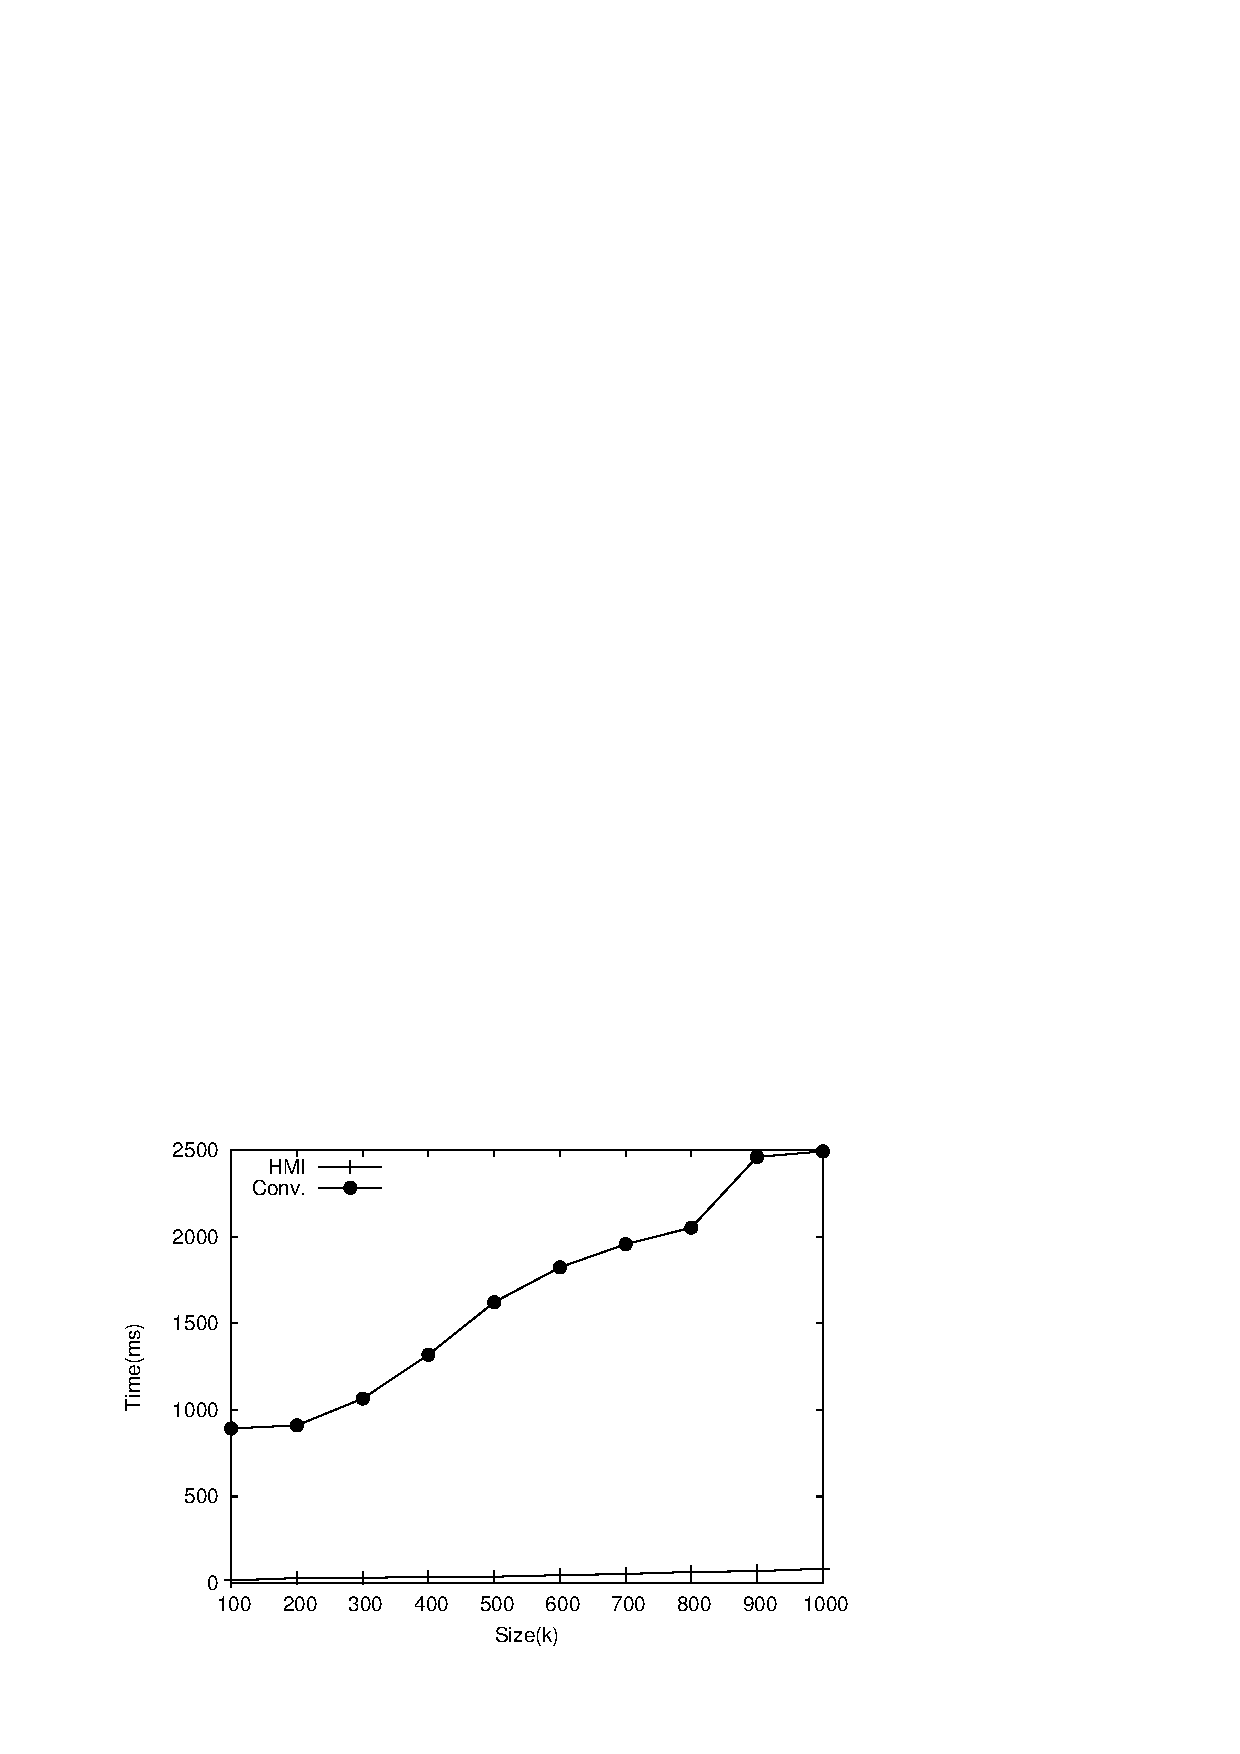
\includegraphics[width=1.5in]{figs/expr/pdf/g_scal_l0i100.pdf}}

%\caption{Scalability}

%\end{figure*}
%\begin{figure*}
%\center
%\subfigure{
%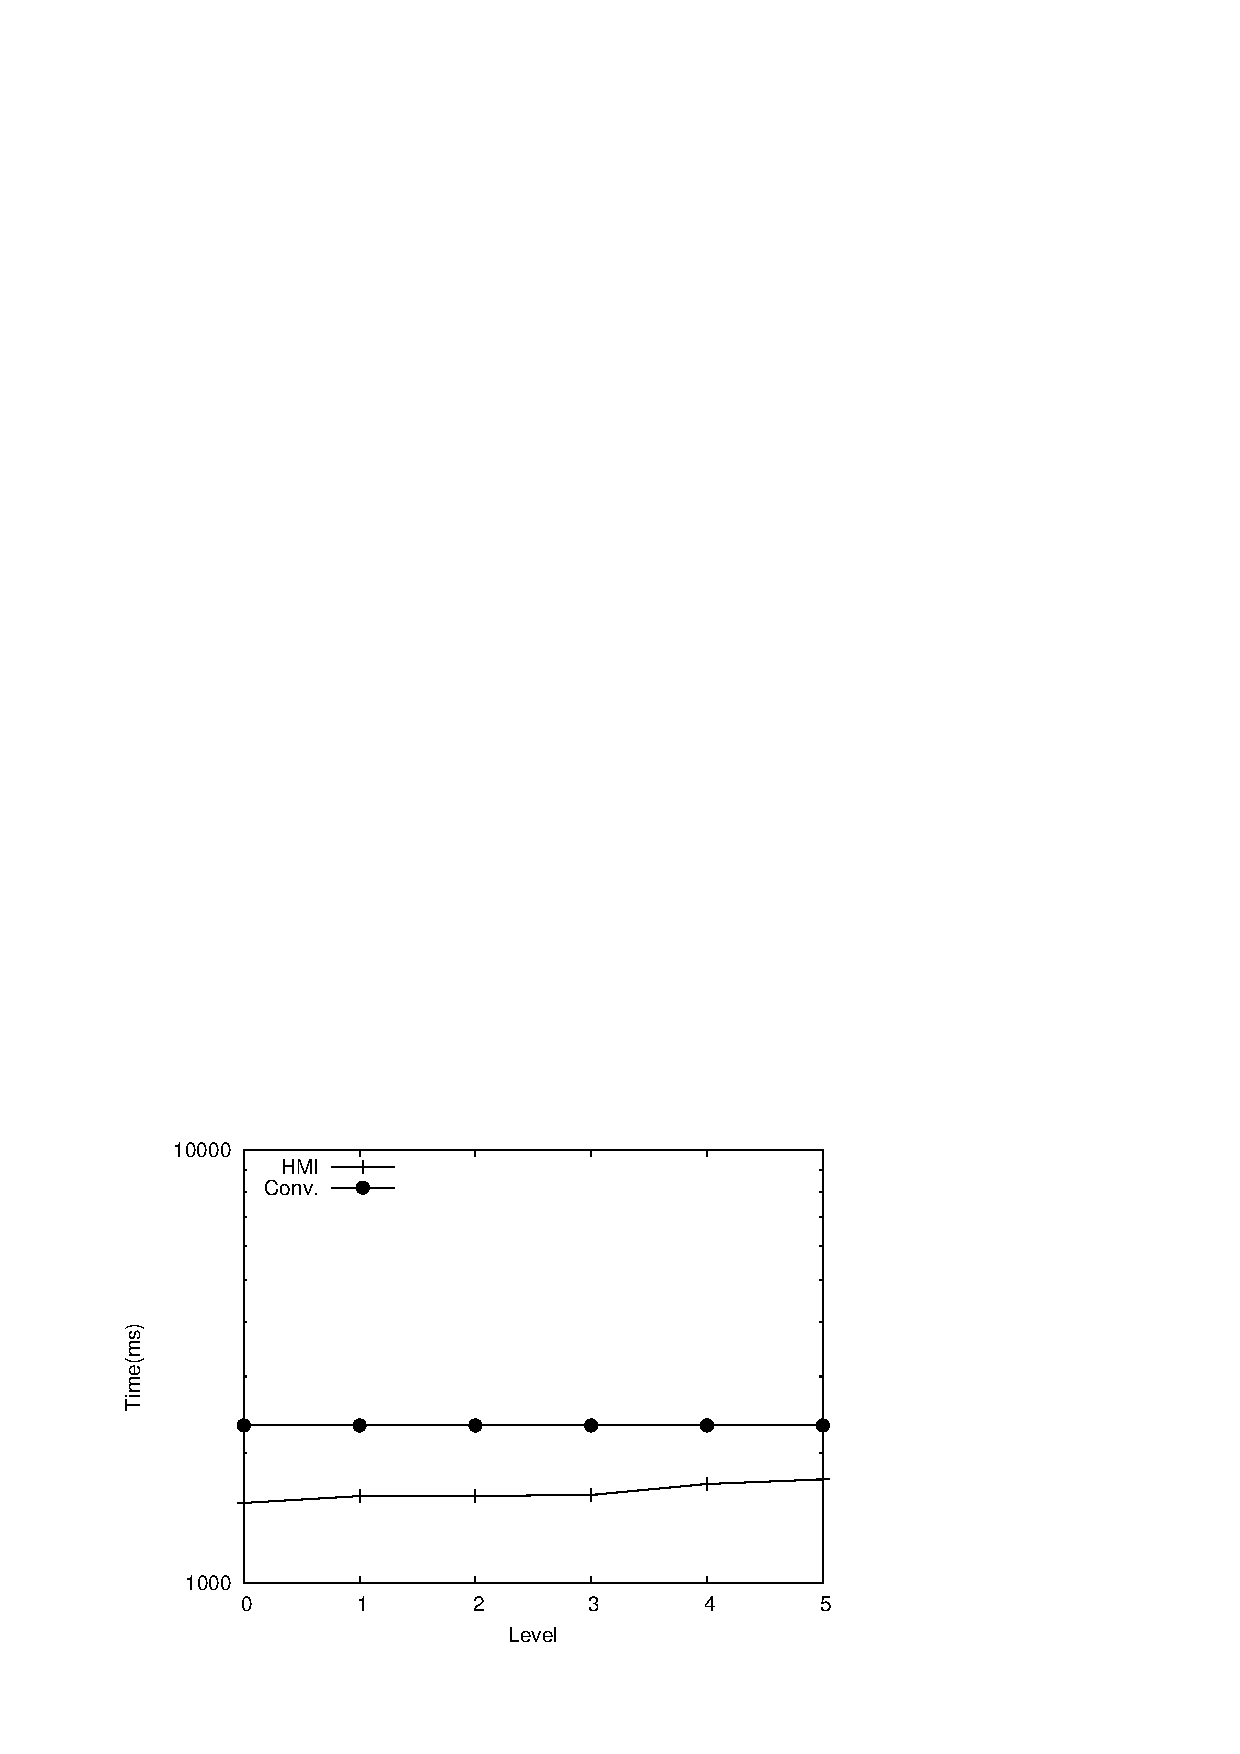
\includegraphics[width=2.0in]{figs/expr/pdf/g_layers_i2.pdf}}
%\subfigure{
%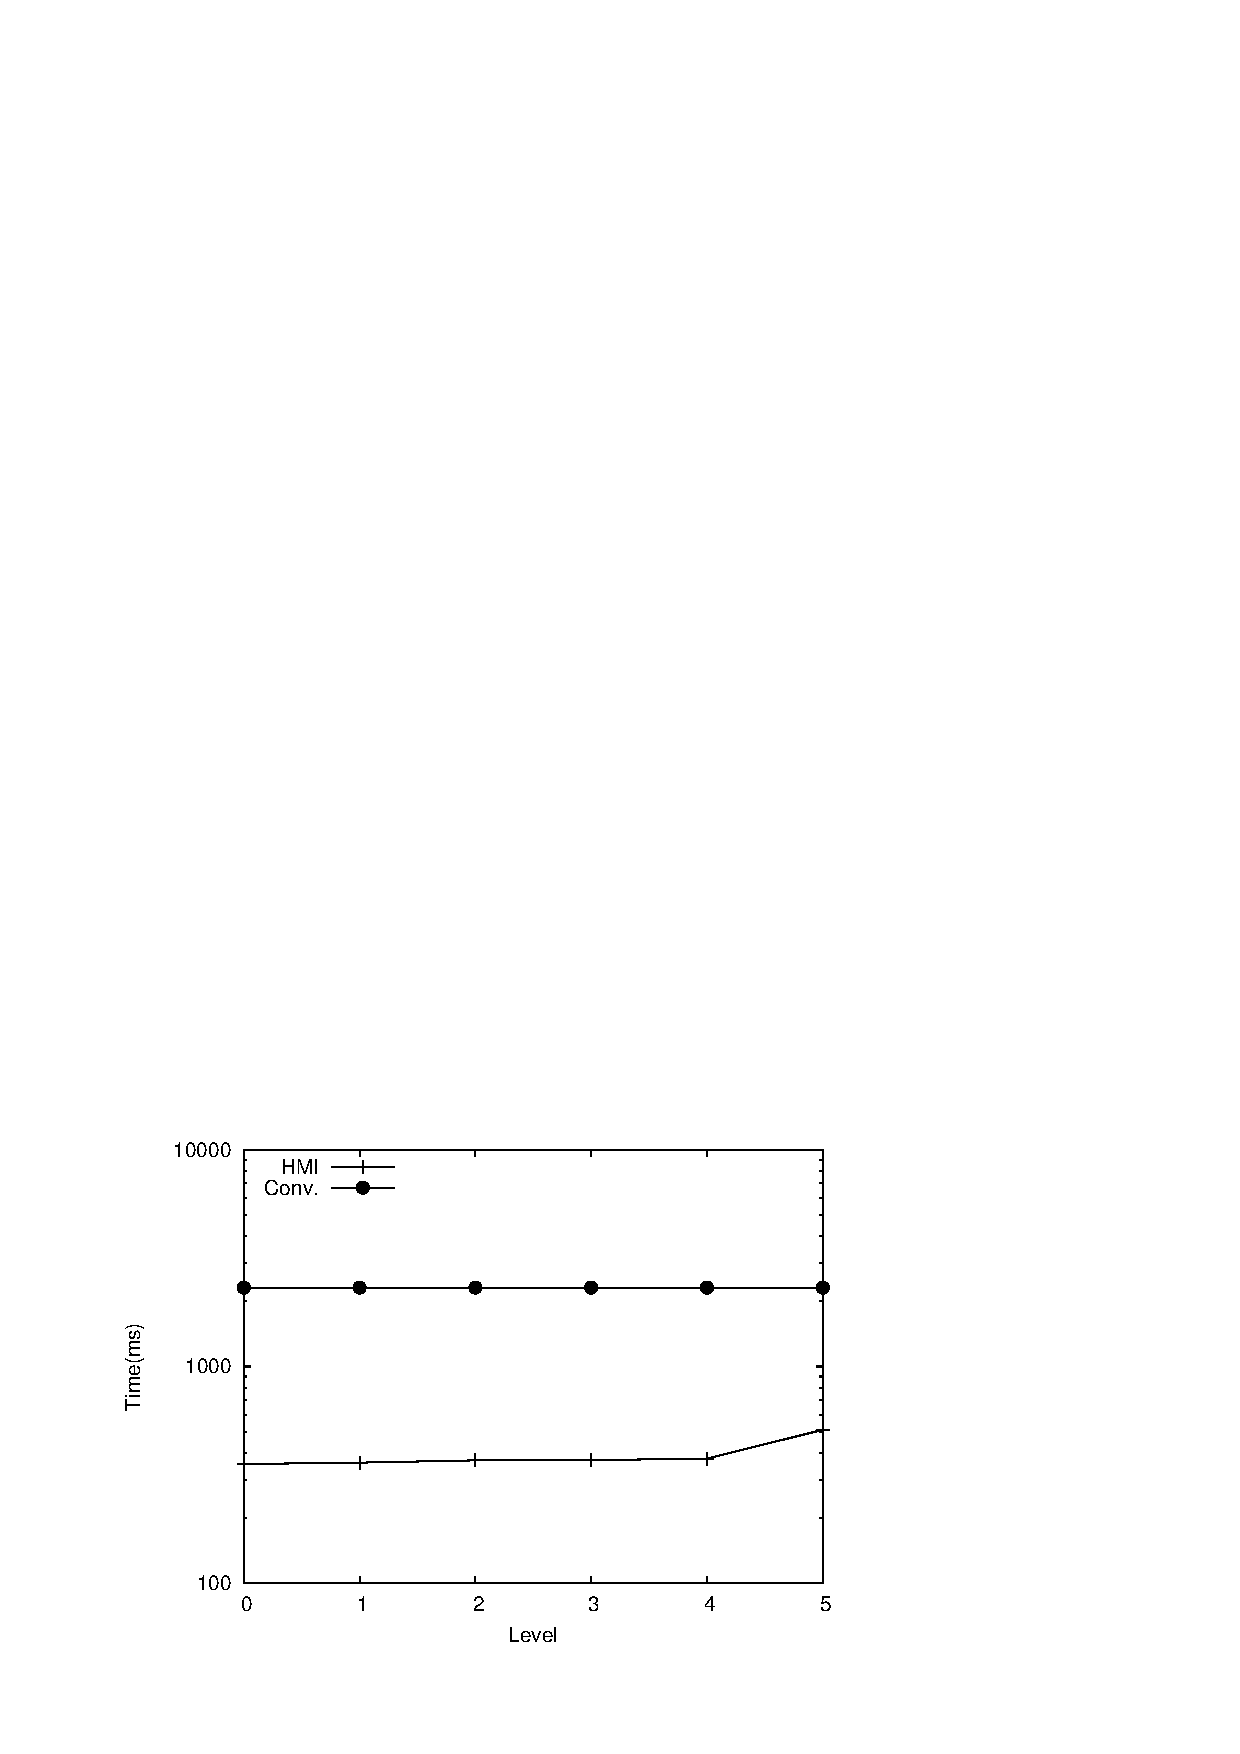
\includegraphics[width=2.0in]{figs/expr/pdf/g_layers_i10.pdf}}
%\subfigure{
%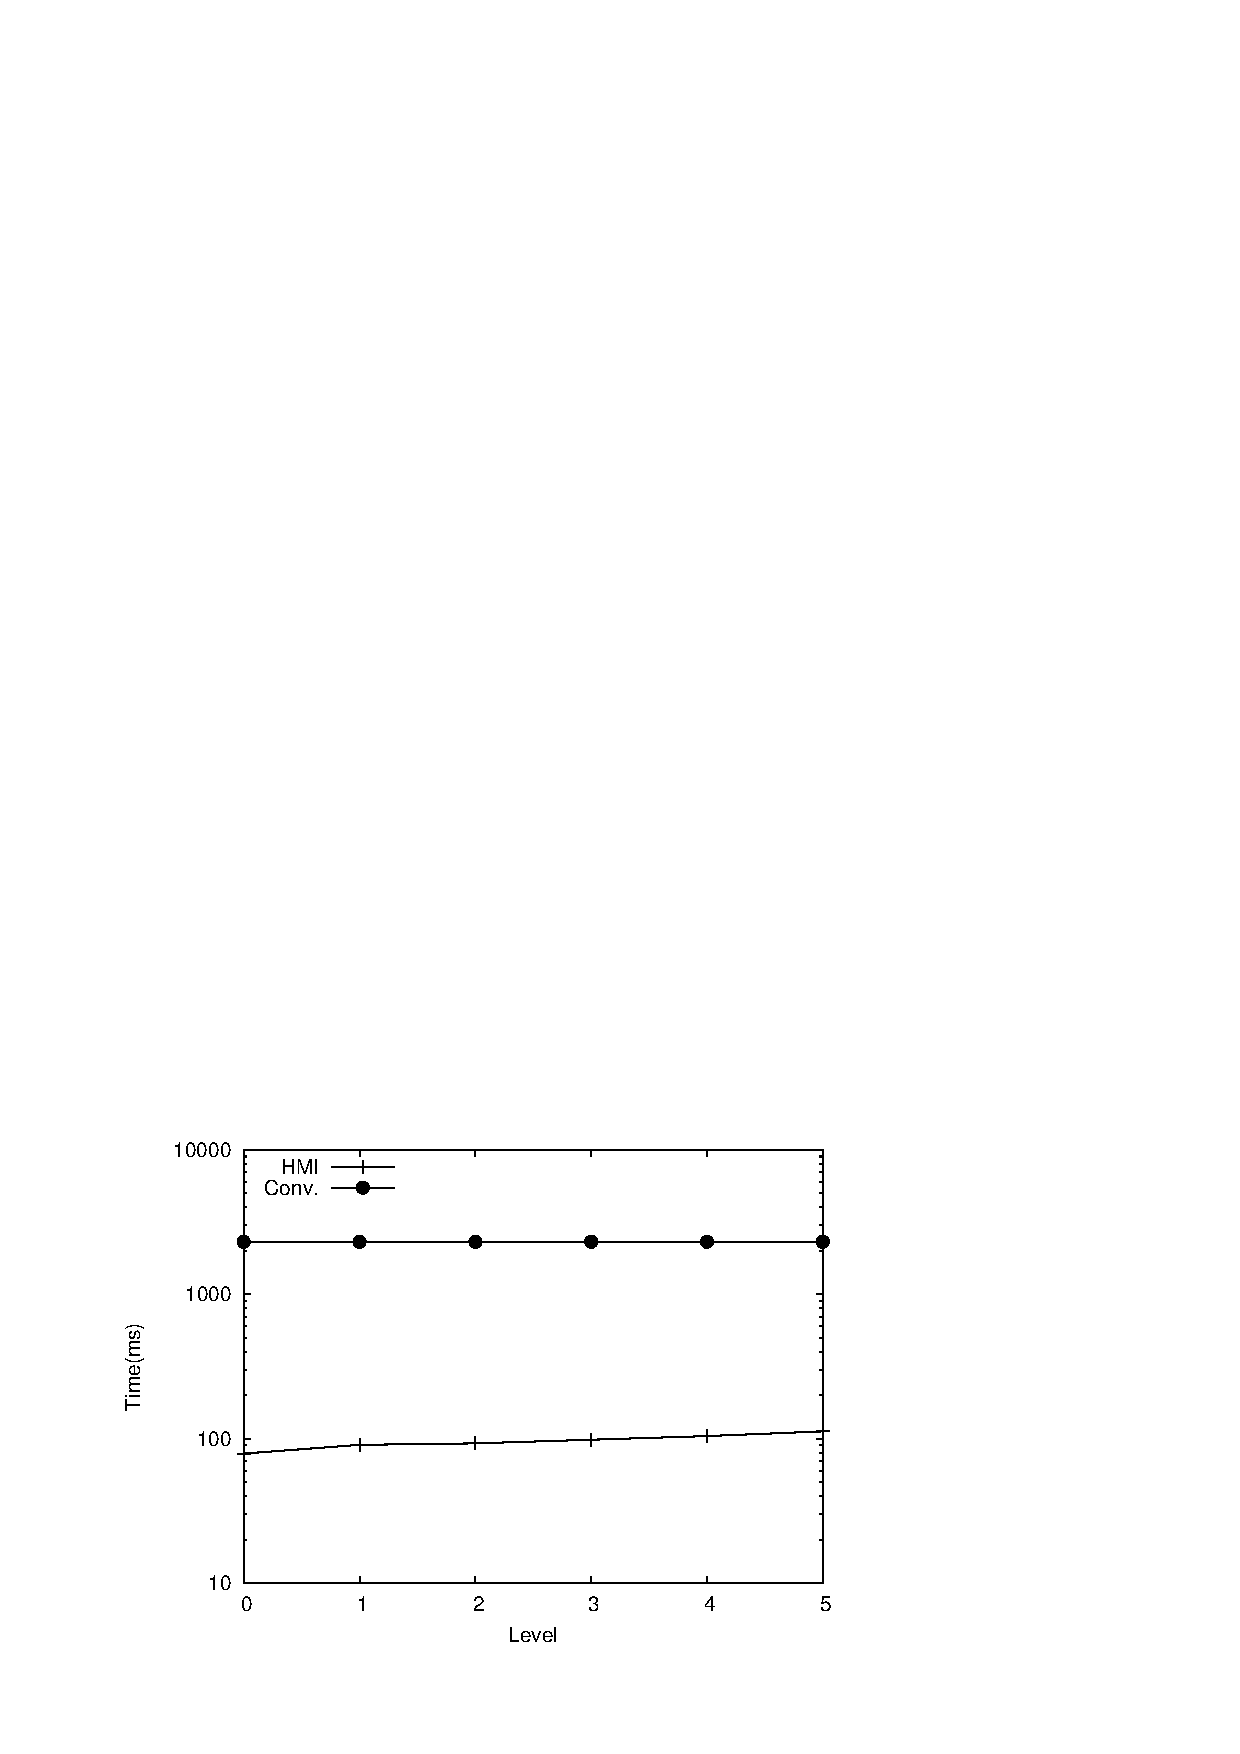
\includegraphics[width=2.0in]{figs/expr/pdf/g_layers_i100.pdf}}
%\caption{Levels in HMI}

%\end{figure*}

%\begin{figure*}
%\center
%\subfigure{
%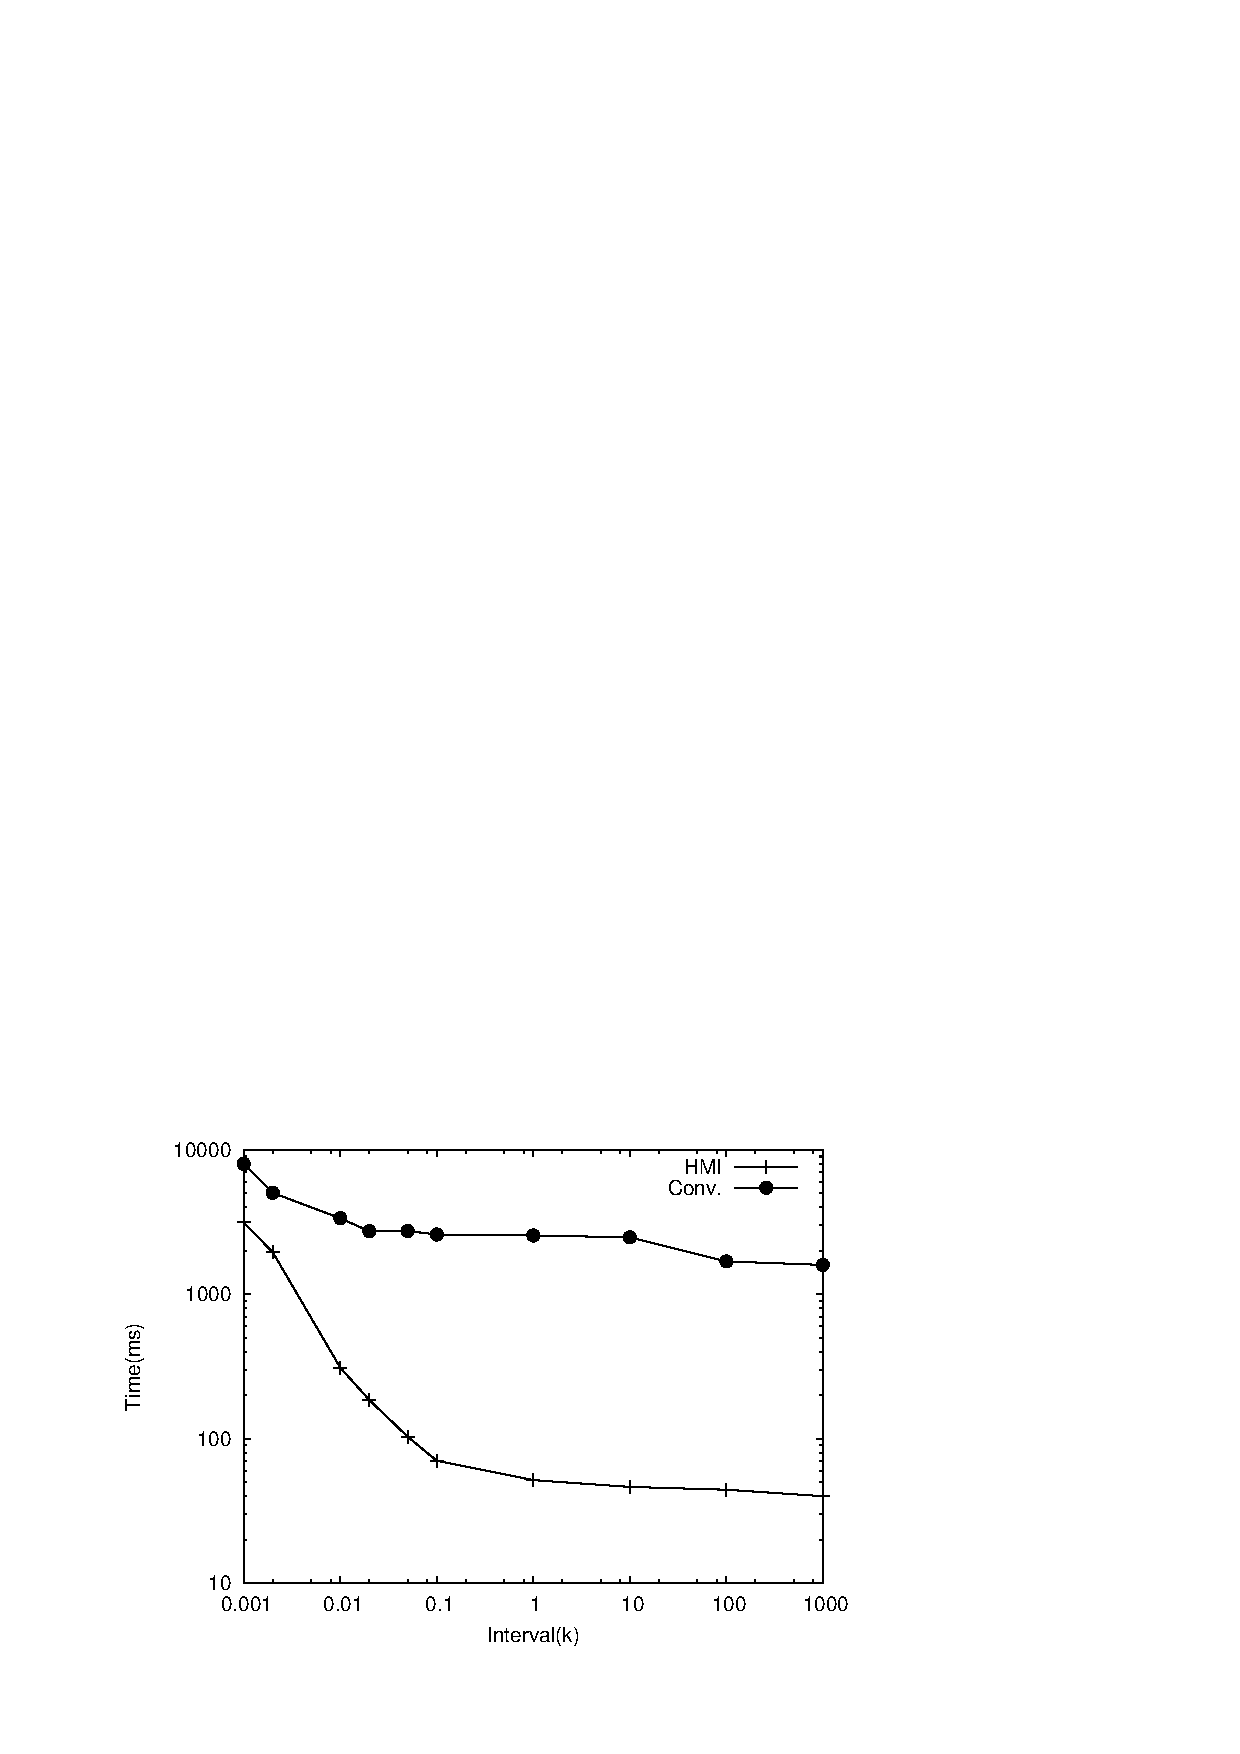
\includegraphics[width=2.0in]{figs/expr/pdf/g_interval_l0.pdf}}
%\subfigure{
%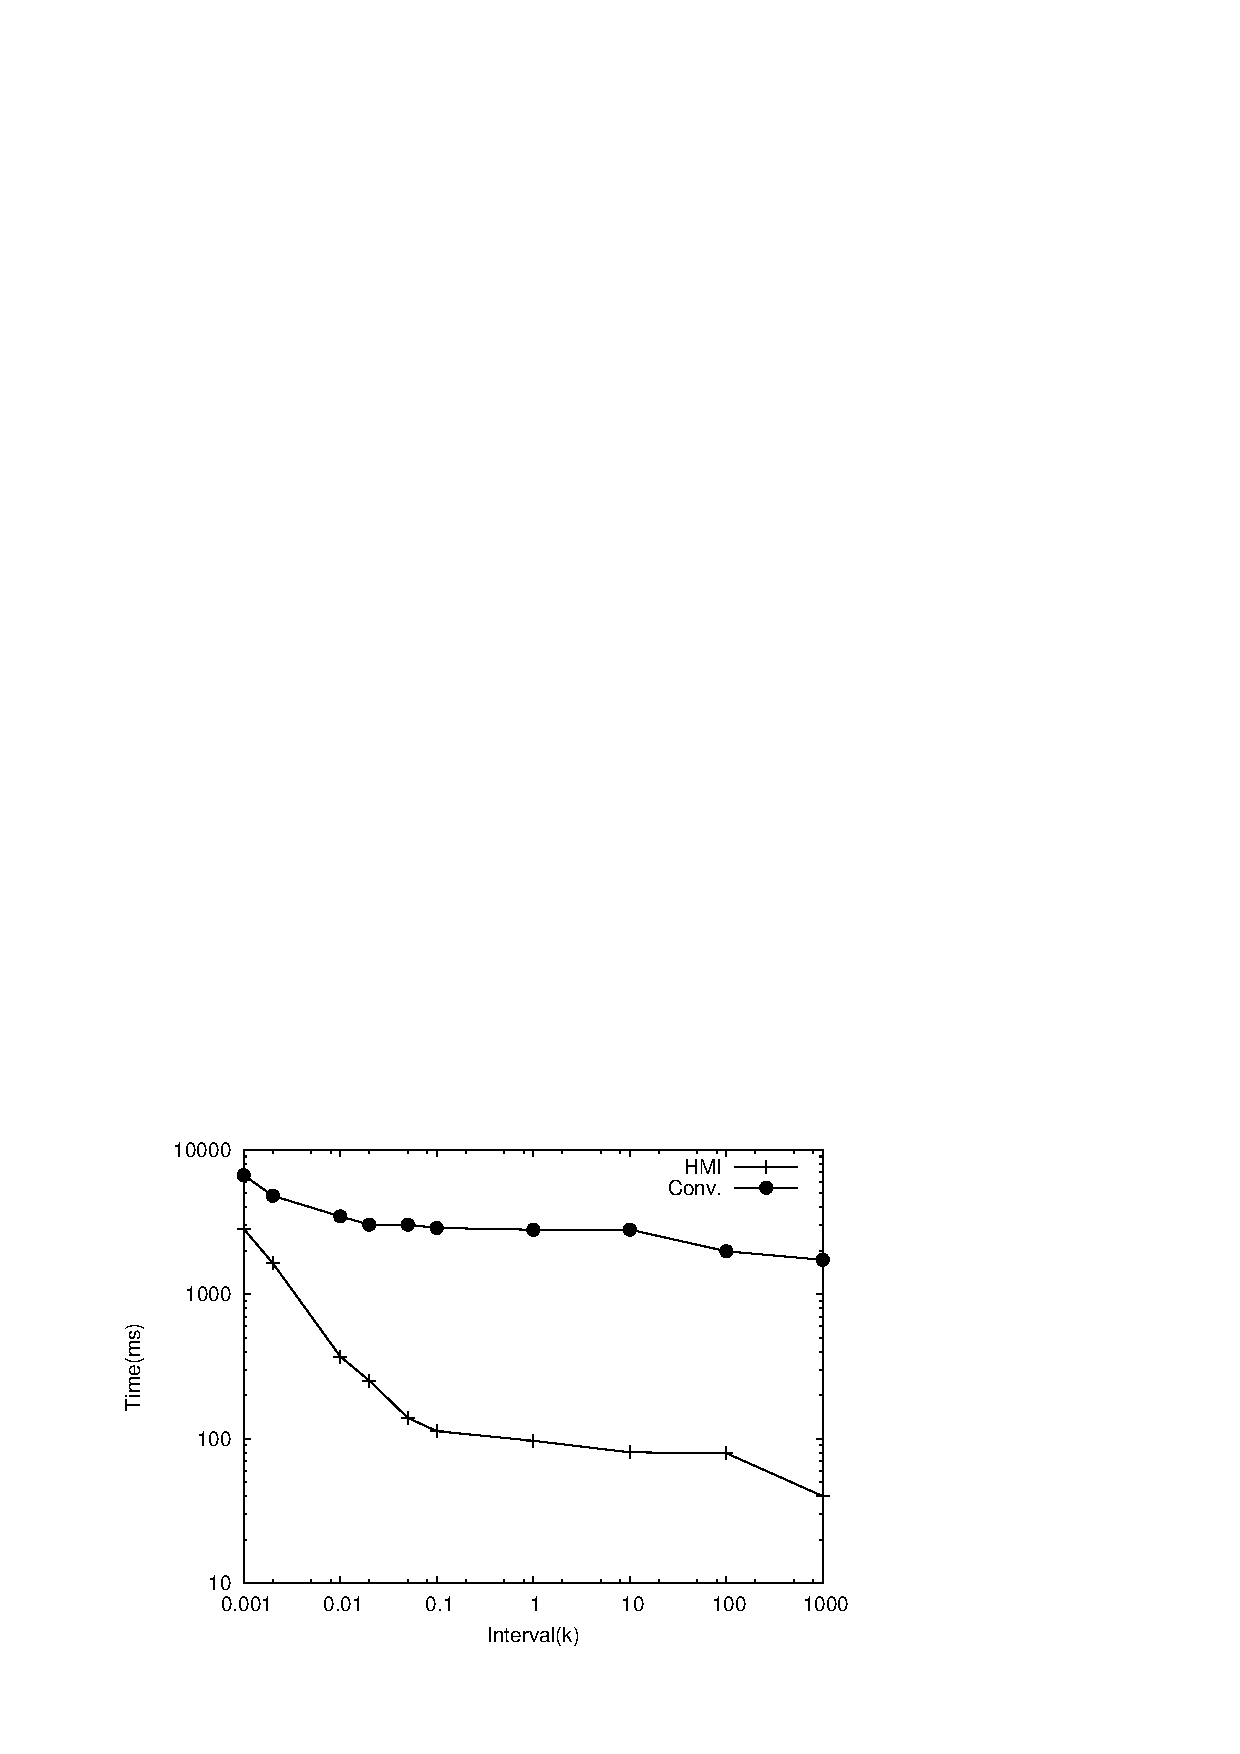
\includegraphics[width=2.0in]{figs/expr/pdf/g_interval_l1.pdf}}
%\subfigure{
%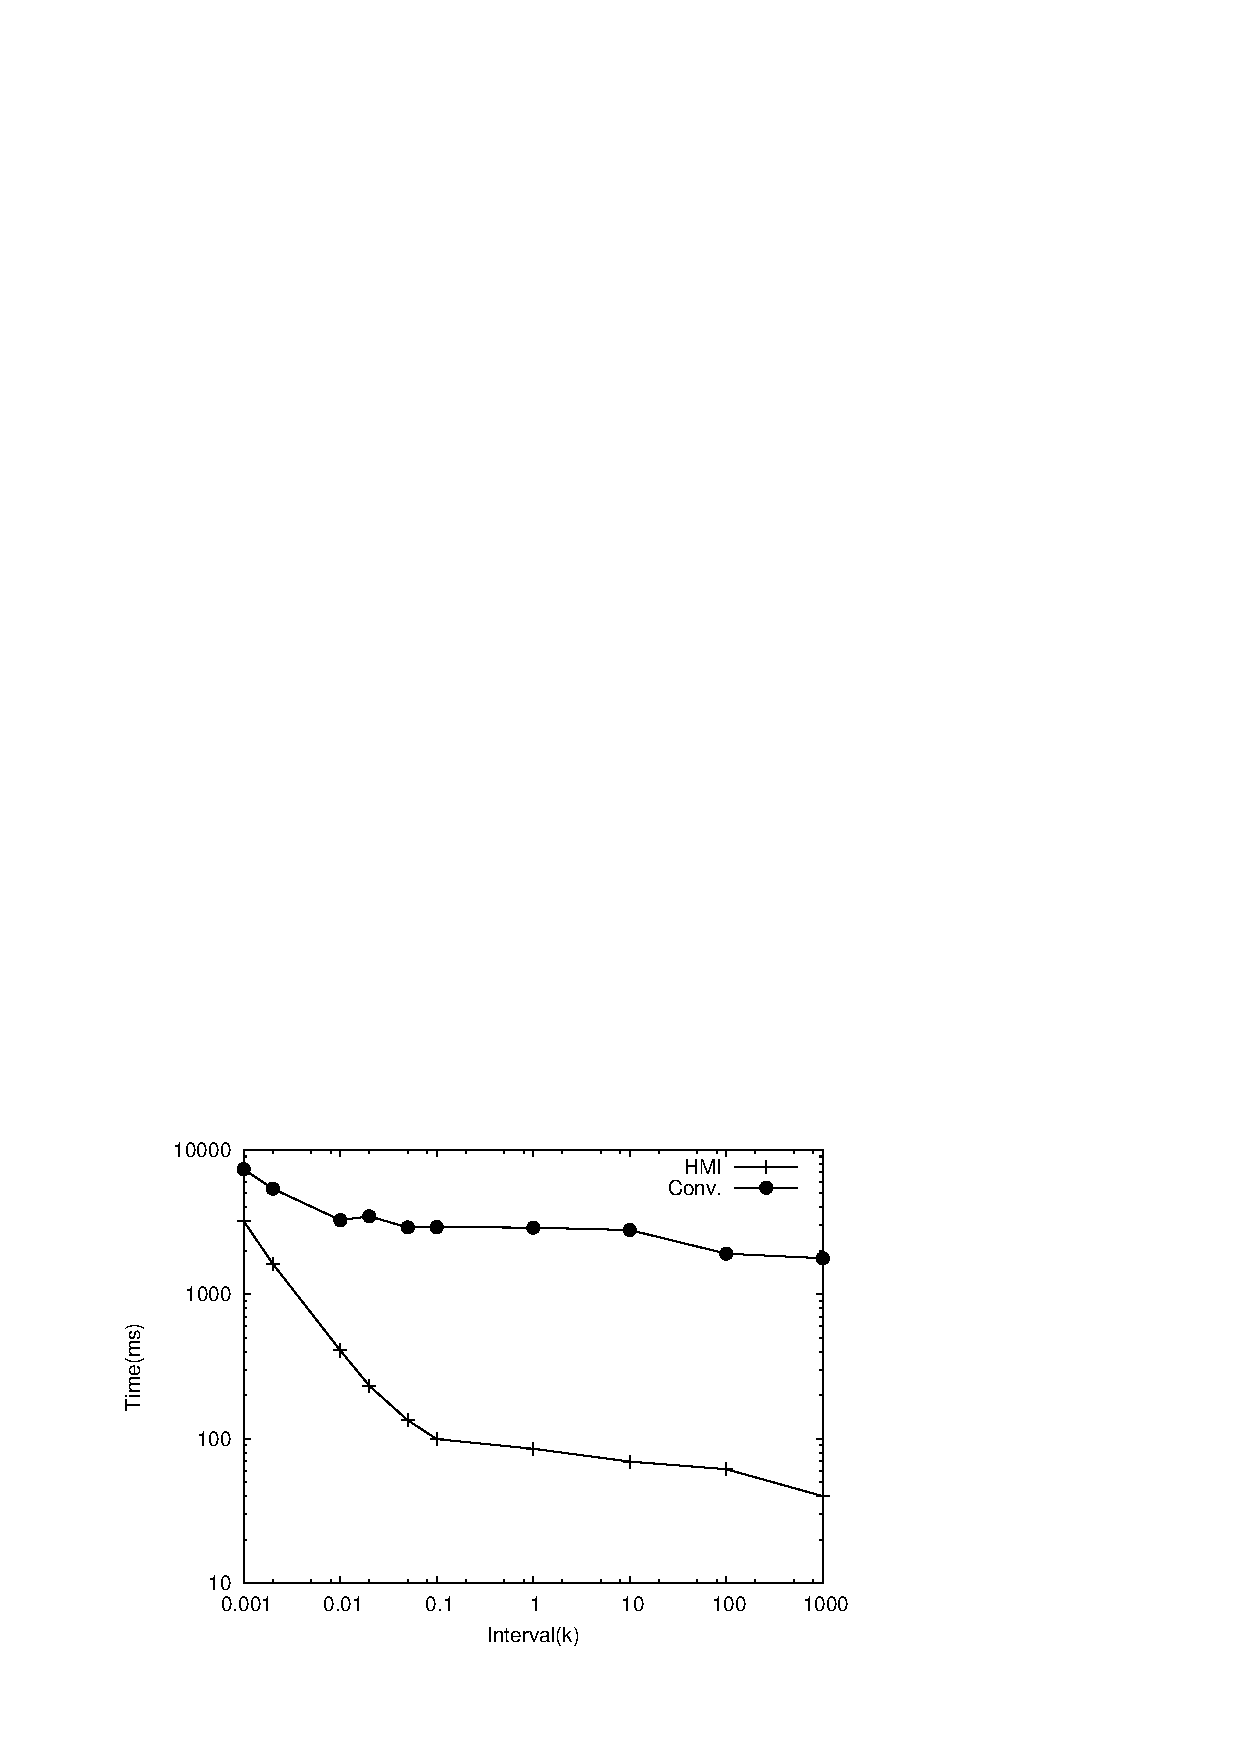
\includegraphics[width=2.0in]{figs/expr/pdf/g_interval_l2.pdf}}
%\caption{Effect of Intervals}

%\end{figure*}

%\begin{figure*}
%\center
%\subfigure{
%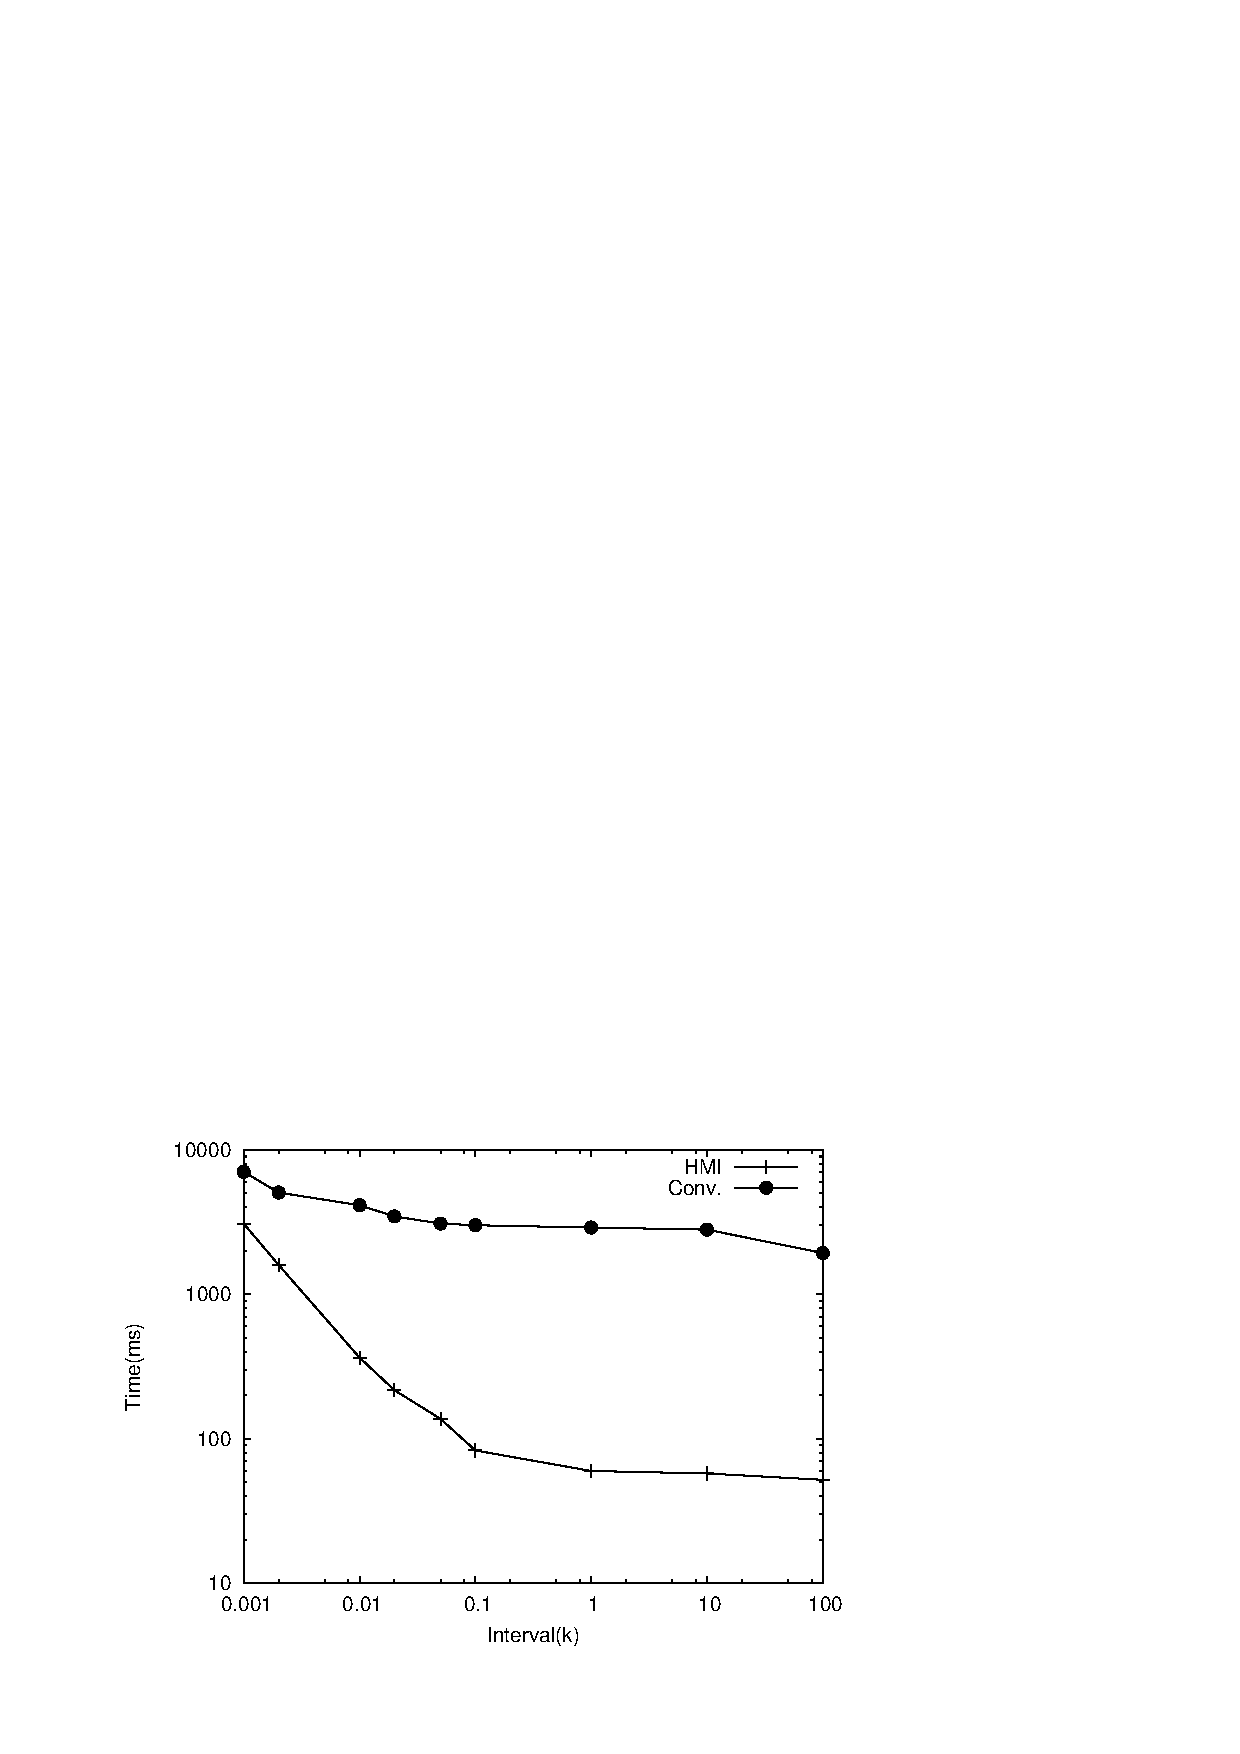
\includegraphics[width=1.5in]{figs/expr/pdf/g_forecast_MA_l0.pdf}}
%\subfigure{
%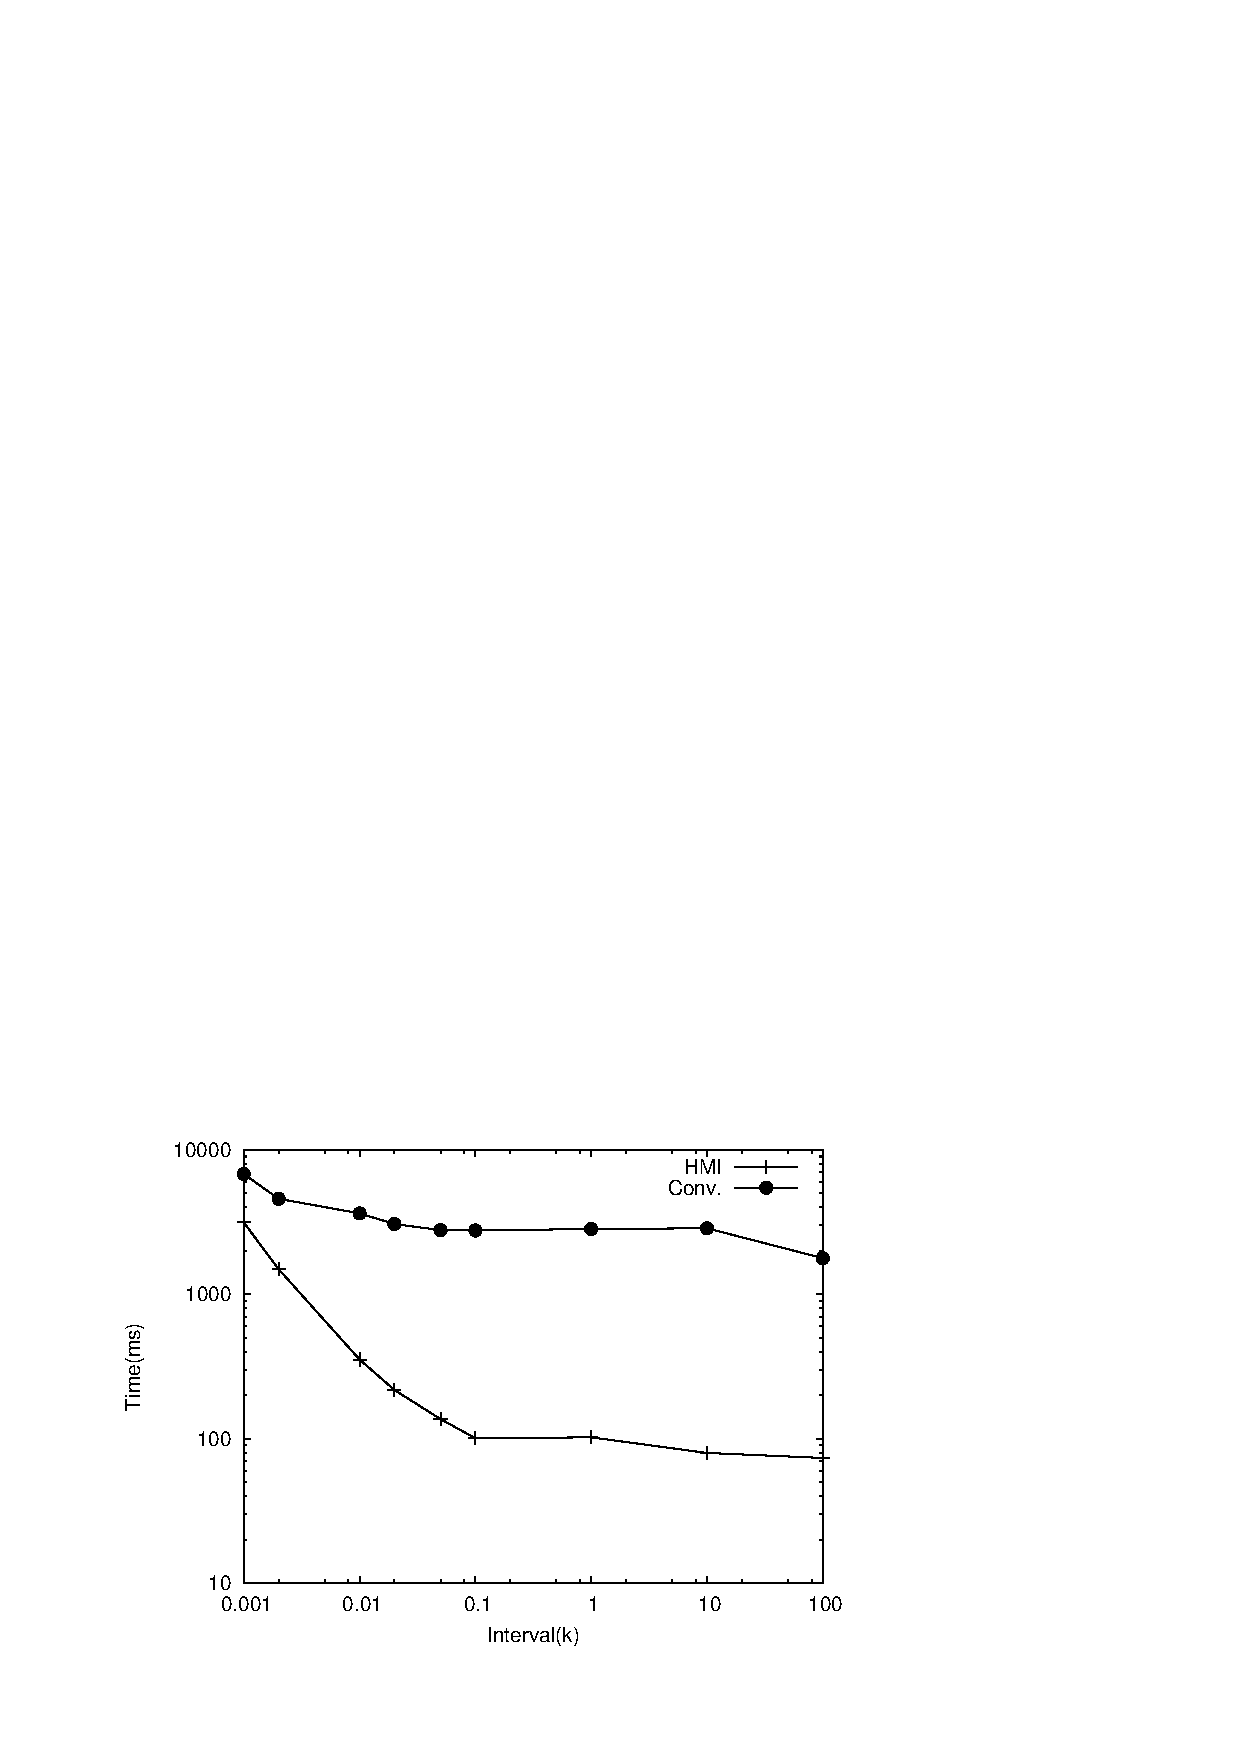
\includegraphics[width=1.5in]{figs/expr/pdf/g_forecast_MA_l1.pdf}}
%\subfigure{
%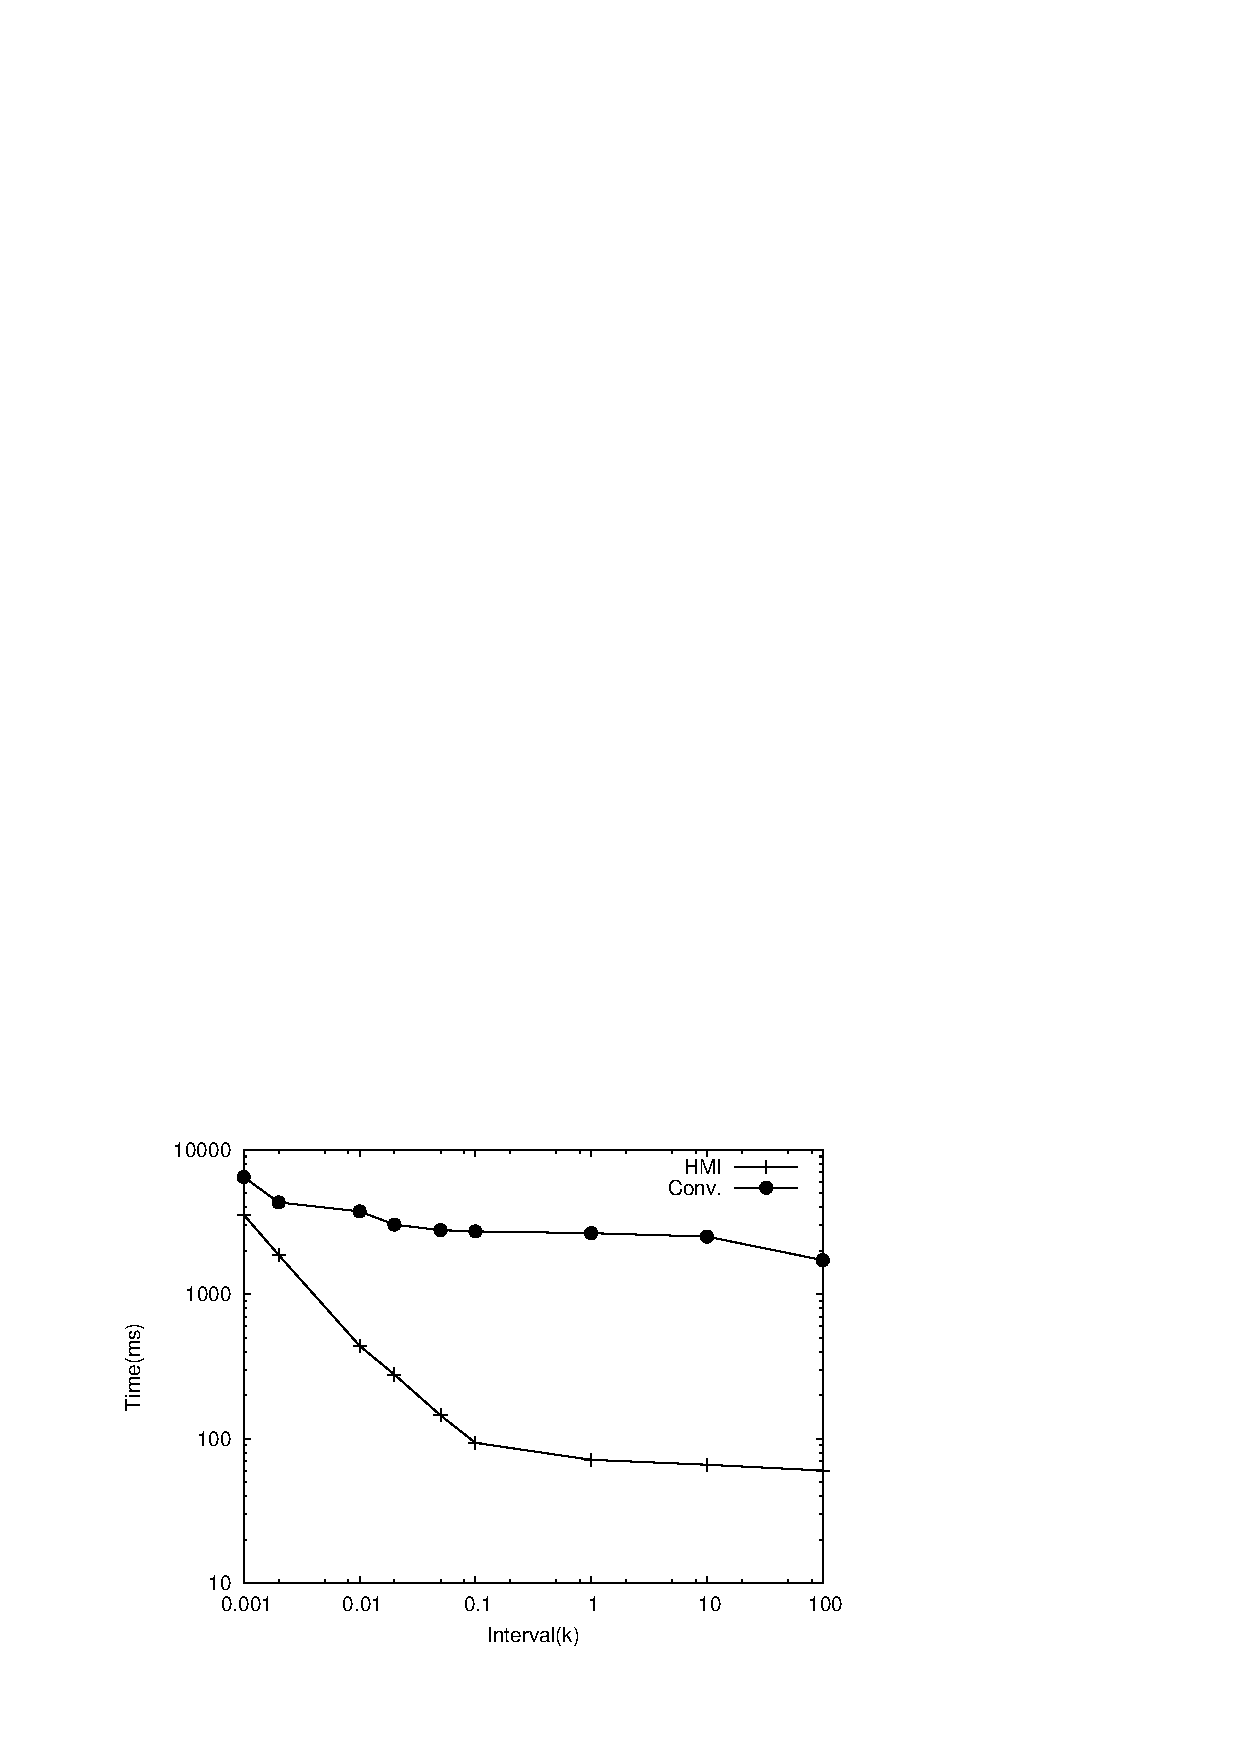
\includegraphics[width=1.5in]{figs/expr/pdf/g_forecast_AA.pdf}}
%\subfigure{
%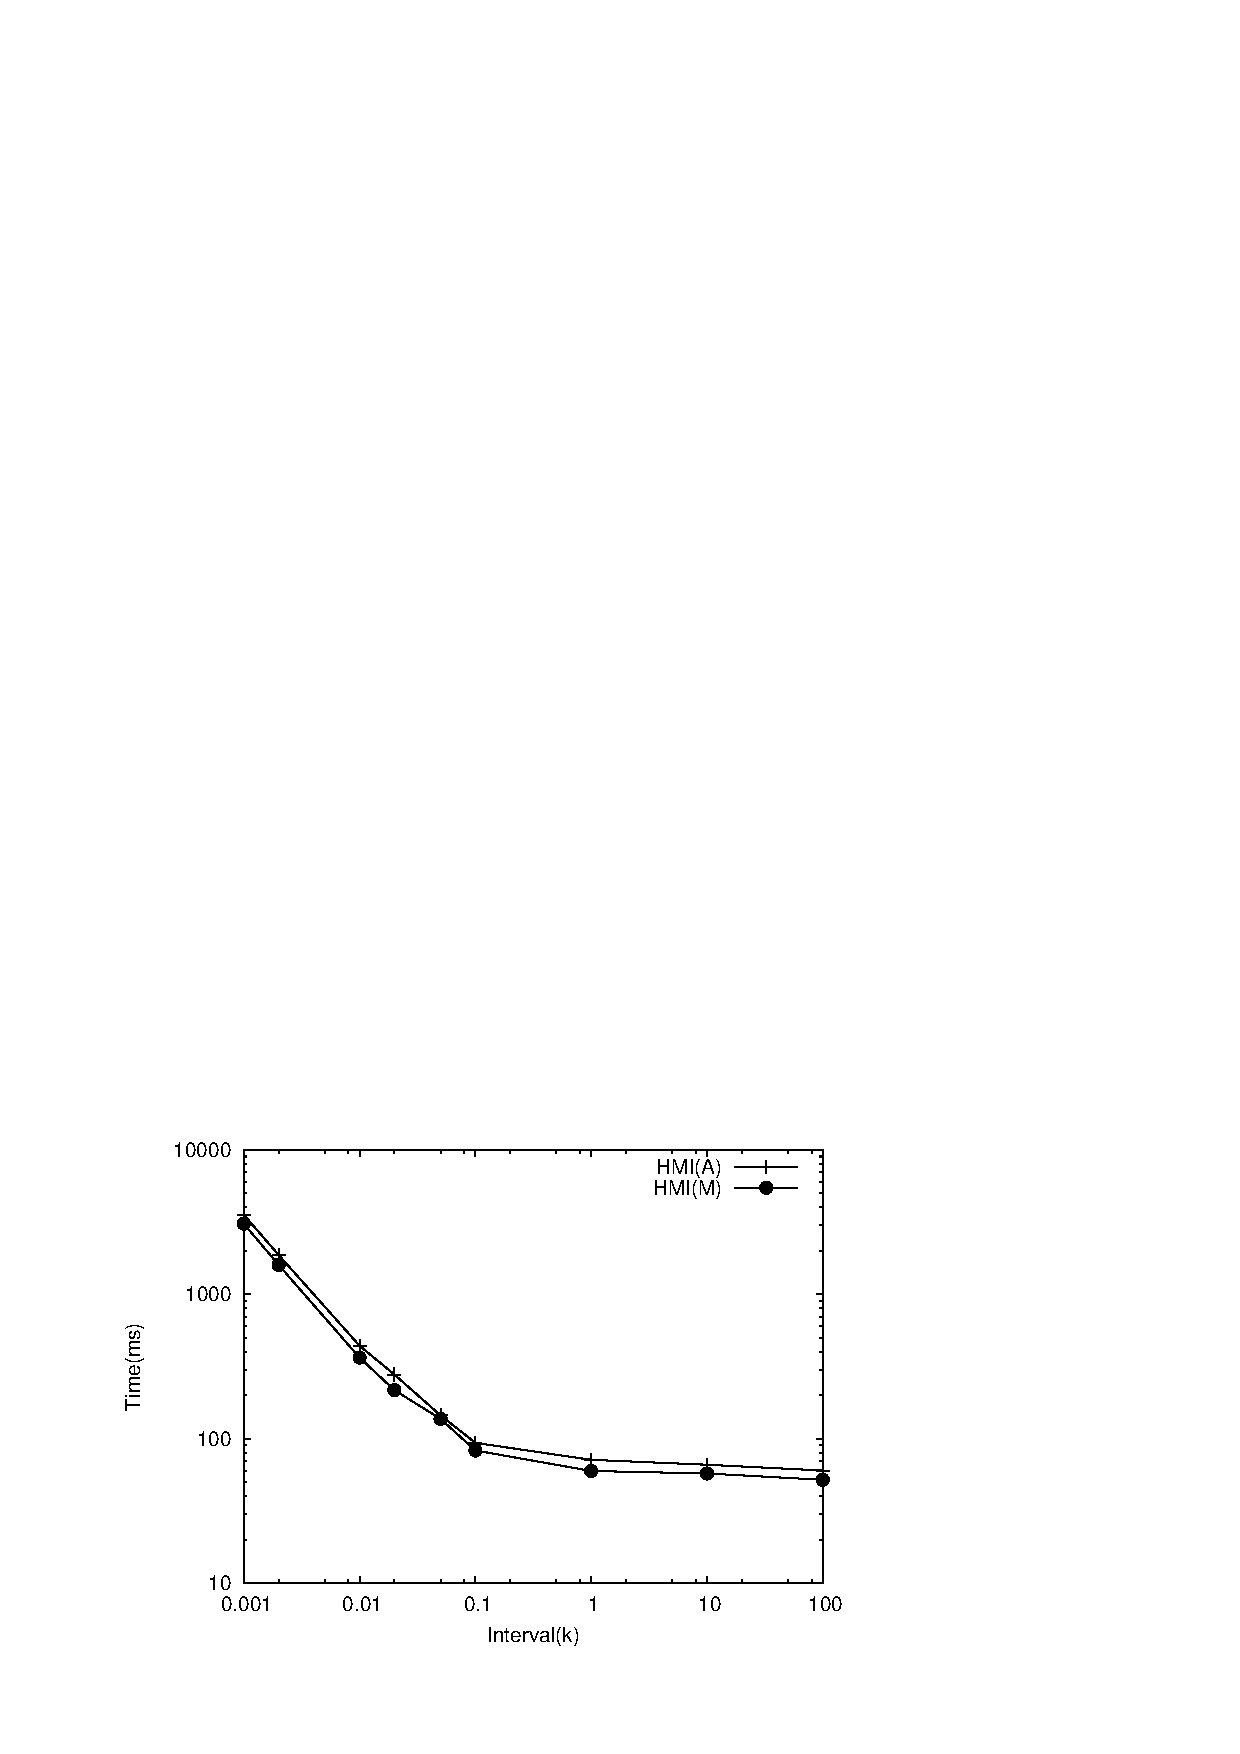
\includegraphics[width=1.5in]{figs/expr/pdf/g_forecast.pdf}}

%\caption{Forecast}

%\end{figure*}



Building model tree and compressing
scaliblity done
inceremental (not yet)
Query done paritally
	Past 
	future
	combined
	add an experiemnts with the number of values size for each level	

\section{Conclusion}
\label{sec:conclusion}
%To acheive that model error, 
%In this paper, we seamlsy integrate historic data and forecasted data. User speci



%Error in forecasted and historic data

%different models paratamer with time (versions of model)

%differnt plans 

%different models on each subset

%use mdoel as an index 

%storing error model

%contexts 


%Future work query optimzer using histogram to ide

% The following two commands are all you need in the
% initial runs of your .tex file to
% produce the bibliography for the citations in your paper.
%\vspace{-10mm}
\bibliographystyle{abbrv}
\scriptsize
\bibliography{demo} 
\end{document}


%Our proposed system consists of the following modules:
% At level $l$, we represent the underling time series $y$ using one or more models ($M^l_1$,$M^l_2$,$\dots$). The error of model $\epsilon(M)$ over interval $I$ is defined as the $l$-maximum absolute difference between the time series data point $y(t)$ and the modeled value $\hat{y}(t)$, where $l$=(1-$\delta(M)$) * $|I|$, the confidence of the model is $\delta(M)$.  Similarly, we compute the error of level $l$, $\epsilon(M)$. As we traverse down the hierarchy,  the error decreases and the confidence increases. 

% For a  model $M$ at level $l$  in the index, we need to determine the interval  range, the upper bound of the error,  the lower bound of confidence, and  branching factor, i.e., the maximum number of intervals at level $l-1$  that are defined over the same interval range.

%find the ''best'' \LN that minimizes the  run time of expected workload while complying with  the specified  storage overhead.

   %determines the interval range, error, confidence, and parameters for each model in the index
%the details of processing  of trend, seasonality, and error components. 

%Hence, the search space to find the best models is large.  User gives hints to specify parameters for the index and  time series to  reduce the search space. We introduce a metric denoted as the model utility. The utility model for $m$, $U(m)$, is the  speedup of expected workload using  model $m$ and its children  models is relative to the storage space needed. % We use  parameters of trend or seasonality to find the similarity between models.   %Section~\ref{sec:compression} gives the details of this module. 


 %For historical queries,  it traverses down the \LN until    the answer meets the user requirement of error guarantee or the underlying time series is  accessed.
%For forecast queries,  we use the forecasting module to retrieve the  predicted the time series.  The forecasting module uses the values of historic data supplied by query processing module and forecast method parameters.

%we use the model at level $n$ ( i.e., the highest level in the hierichy) to obtain an approximate answer for the query. If the answer violates the user requirements of the error and  the confidence, we consult relevant models at level $n-1$ to minimize the error and maximum the confidence.
%If and  using the ranges  of  values retrieved from model index, we can arbitrary shrink the ranges by traversing the hierarchy. 
%For historical queries, we start with the highest level $n$  We continue traversing the in-dex hierarchy until either the user requirement is met oAssume we compute the selWe traverse the hierircal down 
% We reduce the error We reduce the We find more accurate approximate ,  we first use query processing module to find more accurate  data of historic values. Then, we  increase the confidence then we 
%The goal of model maintenance is to provide a logicalconsistency between a time series and the models that are based on it. The most expensive part in model maintenance is parameter estimation, since estimators for typical time series models are implemented using numerical procedures and involve optimization algorithms that evaluate complex cost functions many times over all available data of the time series. To address this issue,

%We use the parameters andThe It  by the the  reposnisble for computing the uses the values of historic data supplied by query processing module and forecast model parameters.


%The main idea (center down in Figure~\ref{fig:arch}) is to use  a  hierarchical  model structure to facilitate  answering approximate queries and indexing the time series.
%The models at the highest level decompose the time series into three components: trend, seasonality, and error.




 % By using these models, we  facilitate computing approximate results within a user-specified error guarantee.

%in an order-of-magnitude of the  response time required by directly access the time series.
%compute the result.

%For example, consider  minimum aggregation queries, we only access the portion of the time series where the minimum value might exists. 

%, in order of   magnitude the responses time for counterpart of result for past and future  queries approximately within  error guarantees (i.e., absolute error and confidence).  in order of  magnitude of the  response time.  
%We demonstrate a scalable database system that   answers   past and future queries on real-world time series, e.g., energy domain. 
%As the time series are usually long~\cite{isax2}, our proposed system  represents them compactly using  models. 
%By using models, our proposed systems answers approximate queries (on past and future data) within  error guarantees (i.e., absolute error $\epsilon$ and confidence $\delta$) in order of  magnitude of the  response time.  Moreover, it efficiently supports historic exact  queries by only accessing   the relevant portions in the specified range of the time series. This is unlike existing approaches which accesses the entire range of the time series to  exactly answer the query.

%To realize this system,  we propose a novel \LN structure. As real-world time series  usually exhibits seasonal behavior, each model in this \sn stores  trend and seasonal components. User specifies  seasonality period, and different error guarantees levels, used forecast method (e.g., ARIMA) and upper limit on the required storage space. We use this information  to build  the \LN. Then, the system incrementally updates the  index and answer approximate and exact queries.
%In the demo, we  show building  the \LN for a real-world time series.   the effect of varying the error guarantee on the speed up for approximate queries and  exact queries.


%The proposed index supports range, point 
%For queries on future data, we use  statistical  forecast methods which use states (i.e., past values) and parameters.  Approximate answer,  which usually sufficient for the user, can be computed in order of magnitude faster than their  counterpart exact queries. Our proposed system supports approximate and exact queries. For approximate answer, user specifies error  guarantees on the reported result. 
%i.e., an upper bound on the error, $\epsilon$ and lower bound on confidence $\delta$, i.e.,  Pr ($ans_{approx}$ $\in$  [ $ans-\epsilon$, $ans+\epsilon$]) $>$ $\delta$, where  $ans_{approx}$ and $ans$ are the  approximate and exact answers respectively.

%(2)~expected workload, (3)~error and confidence levels, (4)~the upper bound on the storage size of the index, and (5) the forecast method (e.g., ARIMA).  
% As there are several possible ways to divide the time series,  we introduce a metric denoted as the model utility to find best models. The model utility  is  the speedup on  expected workload with and without this model . 


%Based on the model error, 
%we divide the time series into non-overlapping sub-intervals $I_i$ (e.g., using approaches in \cite{functionDB,Shatkay}). 
%The user specifies hints for the seasonal period hierarchy.
%For an hourly time series, Figure~\ref{fig:hints} shows two possible hints for seasonality. The first hint should be used if the shape of the time series is similar per year, week and day.  
%If the daily shape for weekdays differs from that of weekends, using the second hint reduces the approximation error.
%To build model segment $m$ over interval $l$, we first decompose the portion of time series over this interval into {\em trend} $t$, {\em seasonal} $s$, and {\em remainder} $r$ components using the longest seasonal period $p$ in the hierarchy, such that the length of the interval is at least  twice $p$. Then, we process each component as described  later. 
%To find the best model representation, we maximize a heuristic, $H$, based on the computed sub-intervals and the size of the model.  Heuristic, $H$, is defined as $(\sum {e_i * |I_i|})/s$, where $|I_i|$ is the length of sub interval $I_i$, $e_i$ is the number of error guarantees levels which complies with interval $I_i$, and $s$ is the model size.
